\documentclass[conference]{IEEEtran}
\IEEEoverridecommandlockouts
\usepackage[utf8]{inputenc}
\usepackage[T1]{fontenc}
\usepackage{amsmath,amssymb,amsfonts}
\usepackage{graphicx}
\usepackage{booktabs}
\usepackage{cite}
\usepackage{algorithm}
\usepackage{algorithmic}
\usepackage{subcaption}
\usepackage{xcolor}
\usepackage{enumitem}
\usepackage{placeins}  % provides \FloatBarrier
\usepackage{hyperref}
\usepackage{tikz}
\usepackage{pgfplots}
\pgfplotsset{compat=1.18}
\usetikzlibrary{shapes.geometric, arrows.meta, positioning, calc, fit, backgrounds, patterns, decorations.markings}
\tikzset{
  block/.style={rectangle, draw, fill=blue!8, text width=2.2cm, text centered, minimum height=0.9cm, rounded corners=2pt, font=\small},
  bigblock/.style={rectangle, draw, fill=blue!8, text width=3.0cm, text centered, minimum height=0.9cm, rounded corners=2pt, font=\small},
  decision/.style={diamond, draw, fill=yellow!15, text width=1.6cm, text centered, aspect=2, inner sep=1pt, font=\scriptsize},
  arrow/.style={-{Stealth[length=2.5mm]}, thick},
  darrow/.style={-{Stealth[length=2.5mm]}, thick, dashed},
  neuron/.style={circle, draw, fill=orange!20, minimum size=0.45cm, inner sep=0pt, font=\tiny},
}

\newtheorem{theorem}{Theorem}
\newtheorem{proposition}[theorem]{Proposition}
\newtheorem{corollary}[theorem]{Corollary}

%==============================================================================
\title{Neural Move Ordering in IDA* Search:\\ Coordinate Features, Node Reduction, and the Inference Overhead Barrier}
%==============================================================================
\author{\IEEEauthorblockN{Akash Chakraborty}
\IEEEauthorblockA{Department Of Computer Science And Engineering / Sister Nivedita University\\
akashchakraborty694@gmail.com}}

\begin{document}
\maketitle

%==============================================================================
\begin{abstract}
The Rubik's Cube has approximately $4.3 \times 10^{19}$ reachable states, making exhaustive optimal search impractical. We present a solver based on Kociemba's Two-Phase Algorithm with three improvements: (i)~\textbf{multi-solution Phase~1 search}, which explores $K$ Phase~1 endpoints and retains the shortest combined solution; (ii)~\textbf{time-bounded anytime mode}; and (iii)~\textbf{neural move ordering} using coordinate-based features. We prove an \emph{admissible bound paradox} (Theorem~1): using neural predictions as IDA* lower bounds causes an exponential node blowup of $b^{\lceil\epsilon\rceil}$, and show the correct integration is through move ordering. On 200 random cubes, multi-solution search with $K{=}5$ reduces mean move count from 20.77 to 20.35 ($p < 0.001$, Cohen's $d = 0.70$) and increases $\leq$20-move solutions from 28\% to 56\%. For neural ordering, we identify a critical \emph{representation bottleneck}: scalar coordinate features yield 5.6\% prediction accuracy (random baseline), while our 161-dimensional binned coordinate features achieve 83.3\%---a 15$\times$ improvement. This translates to a 2.4$\times$ node reduction in IDA* search on 200 scrambles (Theorem~3), but per-node Python inference overhead negates the wall-clock benefit. We formalize this as the \emph{inference overhead barrier}: neural ordering helps only when per-node inference cost is less than the per-node time saved from reduced expansion (Section~\ref{sec:coord-features}). We resolve this barrier via \emph{lookup-table precomputation}: pre-computing 32\,768 move orderings into a 576\,KB table reduces per-node inference to an $O(1)$ array lookup, largely eliminating the overhead ($K{=}5$ + LUT: 3047\,ms vs.\ 3374\,ms for per-node inference, $1.10{\times}$ speedup, 98.5\% reliability). Architecture experiments confirm the barrier is inherent, not an artifact of model capacity: $3{\times}$ larger models gain only $+3.5$ percentage points accuracy at $+26$\% higher inference cost. The benchmark infrastructure, trained models, and reproducible results are provided.
\end{abstract}

\begin{IEEEkeywords}
Rubik's Cube, two-phase algorithm, Kociemba, IDA*, pruning tables, neural heuristics, move ordering, anytime solver, multi-solution search
\end{IEEEkeywords}

%==============================================================================
\section{Introduction}
\label{sec:intro}
%==============================================================================

\subsection{Background}
The Rubik's Cube, invented by Ern\H{o} Rubik in 1974, has become a standard testbed for combinatorics, group theory, and heuristic search~\cite{joyner2008}. Its configuration space forms a group under face turns; the six faces (Up, Down, Left, Right, Front, Back) generate the group via quarter and half turns. A single standard $3{\times}3{\times}3$ cube has 26 visible sub-cubes (cubies): 8 corners, 12 edges, and 6 face centers. Each corner has 3 visible faces (stickers) and each edge has 2, giving 54 total stickers---the natural input to any computational representation.

The mathematical structure of the cube is remarkably rich. The group of reachable configurations has order
\begin{equation}
|G| = \frac{8! \cdot 3^8 \cdot 12! \cdot 2^{12}}{12} \approx 4.33 \times 10^{19},
\end{equation}
where the factors account for corner permutations ($8!$), corner orientations ($3^8$), edge permutations ($12!$), and edge orientations ($2^{12}$), with a factor-of-12 constraint from parity and orientation sum rules. This enormous state space makes exhaustive enumeration or brute-force search completely impractical.

\subsection{Problem Statement: God's Number}
``God's Number'' is the minimum number of moves required to solve any solvable cube from worst-case positions. In the \emph{half-turn metric} (HTM), where both quarter turns ($U$, $U'$) and half turns ($U2$) each count as one move, God's Number is \textbf{20}. Rokicki et al.~\cite{godnumber} proved this in 2010 by combining group-theoretic coset decomposition with massive distributed computation (35 CPU-years on Google infrastructure). In the \emph{quarter-turn metric} (QTM), where each $90^\circ$ turn counts separately, God's Number is \textbf{26}~\cite{rokicki2014}.

The practical implication is clear: \emph{every} scrambled cube can be solved in at most 20 half-turn moves. However, finding these optimal solutions requires exhaustive search through the vast state space, which is infeasible in real time. This motivates the use of near-optimal algorithms that sacrifice guaranteed optimality for vastly improved speed.

\subsection{Motivation and Contributions}
Kociemba's Two-Phase Algorithm offers a practical compromise: it does not guarantee 20 moves for every instance but typically produces 19--22 move solutions in a fraction of a second. It improves on Thistlethwaite's four-phase method by using two phases and efficient coordinate-based search with pruning tables. This work implements the algorithm and contributes the following extensions:

\begin{enumerate}[leftmargin=*]
  \item \textbf{Multi-solution Phase~1 search} ($K > 1$ endpoints), which explores multiple Phase~1 exit points and retains the shortest combined solution.
  \item \textbf{Time-bounded anytime mode}, which caps solve latency for interactive applications while returning the best solution found within the budget.
  \item \textbf{Neural move ordering with coordinate features}, addressing the representation bottleneck through 161-dimensional binned coordinate features that raise prediction accuracy from 5.6\% to 83.3\% and reduce IDA* nodes by 2.4$\times$.
  \item \textbf{Formal analysis} of the admissible bound paradox (Theorem~\ref{thm:bound-paradox}), multi-solution order statistics (Proposition~\ref{prop:order-stat}), and the inference overhead barrier (Theorem~\ref{thm:node-reduction}).
\end{enumerate}

Validation highlights:
\begin{itemize}[leftmargin=*]
  \item Statistically validated improvements ($K{=}5$: $p < 0.001$, Cohen's $d = 0.70$).
  \item Proof that na\"ive neural bounds cause exponential blowup in IDA* (Theorem~\ref{thm:bound-paradox}).
  \item Identification and resolution of the representation bottleneck: binned coordinate features achieve 83.3\% accuracy vs.\ 5.6\% for scalar features.
  \item Characterization of the inference overhead barrier: 2.4$\times$ node reduction offset by per-node inference cost.
  \item Full open reproducibility (seed, scripts, JSON outputs, trained models).
\end{itemize}

\subsection{Practical Applications}
The Rubik's Cube solver has applications in \textbf{robotics} (minimizing actuator moves in physical solves), \textbf{education} (illustrating group theory and algorithmic concepts), and \textbf{AI benchmarking} (the cube's $4.3 \times 10^{19}$ states with known-optimal baselines make it an ideal testbed for neural heuristics).

\subsection{Paper Organization}
Section~\ref{sec:related} reviews related work. Section~\ref{sec:math} presents mathematical foundations including formal theorems. Section~\ref{sec:method} details our methodology. Sections~\ref{sec:results}--\ref{sec:discussion} present and discuss results. Section~\ref{sec:conclusion} concludes.

%==============================================================================
\section{Related Work}
\label{sec:related}
%==============================================================================

\textbf{Optimal solvers and God's Number.}
Korf~\cite{korf1997} achieved the first optimal solver using IDA*~\cite{korf1985} with pattern databases~\cite{culberson1998}. Rokicki et al.~\cite{godnumber} proved God's Number is 20 in the half-turn metric using 35 CPU-years of computation, establishing the theoretical ceiling for practical solvers.

\textbf{Thistlethwaite and Kociemba.}
Thistlethwaite~\cite{thistlethwaite1981} introduced nested-subgroup reduction ($G_0 \supset G_1 \supset G_2 \supset G_3 \supset \{e\}$). Kociemba~\cite{kociemba} simplified this to two phases with coordinate-based pruning tables, enabling near-optimal solutions in milliseconds. Our work extends Kociemba's algorithm with multi-solution Phase~1 search and neural move ordering.

\textbf{Deep learning for combinatorial puzzles.}
DeepCubeA~\cite{deepcubea} uses deep approximate value iteration with weighted A* to solve optimally in 60\% of cases (median 21 moves), but requires $\sim$2 days GPU training and $\sim$10\,s per solve. McAleer et al.~\cite{mcaleer2018} explored policy gradient methods with less success. Brunetto and Trunda~\cite{brunetto2017} showed that cube-specific architectures are needed for distance estimation---consistent with our finding that feature representation is the bottleneck. More broadly, the success of neural network--guided tree search in games such as Go~\cite{silver2016, silver2017} has motivated applying similar techniques to single-agent search problems.

\textbf{Neural heuristics in planning.}
Shen et al.~\cite{shen2020} showed that even small heuristic errors cause exponential node expansion in IDA*---the ``heuristic noise'' problem that our Theorem~\ref{thm:bound-paradox} formalizes. Ferber et al.~\cite{ferber2022} demonstrated the importance of domain-specific features for neural heuristics in STRIPS planning, supporting our finding that binned coordinate features dramatically outperform raw scalars.

\textbf{Pattern databases and symmetry.}
Felner et al.~\cite{felner2004} developed additive PDB partitioning achieving heuristic values averaging 8.3 moves, stronger than Kociemba's $\sim$5--6 but requiring hundreds of MB vs.\ $\sim$20\,MB. Korf and Felner~\cite{korf2002} introduced disjoint PDBs, and Holte et al.~\cite{holte2006} further extended these with compressed representations. The cube's 48-element symmetry group can further reduce database sizes by $48\times$.

\textbf{Positioning.}
Unlike end-to-end learned solvers (DeepCubeA), we study neural heuristics as \emph{add-ons} to an established classical algorithm, taking inspiration from move-ordering techniques in game-tree search~\cite{schaeffer1989, reinefeld1994}. Our coordinate feature results show this integration \emph{can} yield node reductions (2.4$\times$ on 200 scrambles), but the inference overhead barrier limits practical benefit in interpreted languages. Arfaee et al.~\cite{arfaee2011} showed that bootstrapped heuristic learning can improve heuristic accuracy over large state spaces; our coordinate features achieve a similar goal through engineered features rather than iterative deepening of the training process.

%==============================================================================
\section{Mathematical Foundation}
\label{sec:math}
%==============================================================================

The set of reachable states of the Rubik's Cube forms a group $G$ under the operation of applying one move after another. The full group is generated by the six face turns:
\begin{equation}
G_0 = \langle U, D, L, R, F, B \rangle.
\end{equation}
Each generator admits three non-trivial moves: a clockwise quarter turn ($X$), a half turn ($X^2$), and a counter-clockwise quarter turn ($X' = X^3$). This gives $6 \times 3 = 18$ possible moves at each state, establishing the branching factor for search.

\subsection{Coordinate System}
\label{sec:coordinates}
Rather than storing full permutation arrays, the solver encodes each cube state using compact \emph{coordinates} that capture the relevant symmetry properties:

\begin{itemize}[leftmargin=*]
  \item \textbf{Twist} ($0 \leq \text{twist} < 2187 = 3^7$): Encodes the orientation of 8 corners (the 8th is determined by the others).
  \item \textbf{Flip} ($0 \leq \text{flip} < 2048 = 2^{11}$): Encodes the orientation of 12 edges (the 12th is determined).
  \item \textbf{Slice} ($0 \leq \text{slice} < 495 = \binom{12}{4}$): Encodes which 4 of 12 edge positions are occupied by middle-slice edges.
  \item \textbf{URFtoDLF} ($0 \leq c < 20160 = 8!/2$): Corner permutation coordinate for Phase~2.
  \item \textbf{URtoDF} ($0 \leq c < 665280 = 12!/(12{-}6)!$): Six-edge permutation coordinate for Phase~2.
\end{itemize}

Moves are applied by table lookup: for each coordinate $c$ and move $m$, a precomputed table stores the resulting coordinate $c' = \text{moveTable}[c][m]$. This reduces each move application to $O(1)$ table lookups.

\subsection{Phase~1: Target Subgroup $G_1$}
Phase~1 searches for a path from the initial state (in $G_0$) to a state in the subgroup
\begin{equation}
G_1 = \langle U, D, L^2, R^2, F^2, B^2 \rangle.
\end{equation}
A state belongs to $G_1$ if and only if: (i)~all 12 edges have correct orientation (flip $= 0$), (ii)~all 8 corners have correct orientation (twist $= 0$), and (iii)~the four middle-slice edges occupy middle-slice positions (slice $= 0$). The combined Phase~1 coordinate space has size $2187 \times 2048 \times 495 \approx 2.2 \times 10^9$.

\subsection{Pruning Tables}
\label{sec:pruning}
Pruning tables store the minimum number of moves to reach $G_1$ (or the identity, in Phase~2) from each coordinate value. They are computed by backward BFS from the target:

\begin{itemize}[leftmargin=*]
  \item \textbf{Slice--Twist pruning} ($495 \times 2187$): Lower bound from slice and twist coordinates.
  \item \textbf{Slice--Flip pruning} ($495 \times 2048$): Lower bound from slice and flip coordinates.
  \item \textbf{Phase~2 pruning}: Uses URFtoDLF, URtoDF, and the restricted slice coordinate.
\end{itemize}

The admissible heuristic at any node is $h = \max(h_{\text{slice-twist}}, h_{\text{slice-flip}})$ for Phase~1. This maximum of two projections provides a tighter lower bound than either alone while remaining admissible (since both are lower bounds on the true distance).

\subsection{Phase~2}
From any state in $G_1$, only the 10 moves from the generating set of $G_1$ are used: $\{U, U', U^2, D, D', D^2, L^2, R^2, F^2, B^2\}$. Phase~2 finds a path to the identity (solved cube). The restricted move set keeps the effective branching factor at $\sim$10 (vs.\ 18 in Phase~1) and allows strong pruning via precomputed tables, making Phase~2 searches typically much cheaper than Phase~1.

The Phase~2 coordinate system uses three coordinates:
\begin{itemize}[leftmargin=*]
  \item \textbf{URFtoDLF} ($0 \leq c < 20160$): The permutation of the 8 corners, encoded as an index into the $8!/2$ even permutations (parity is fixed in $G_1$).
  \item \textbf{URtoDF} ($0 \leq c < 665280$): The permutation of 6 specific edges (UR, UF, UL, DR, DF, DL), encoded as a $P(12,6)$ index.
  \item \textbf{Slice (Phase~2)} ($0 \leq c < 24$): The permutation of the 4 middle-slice edges among themselves (all 4 are in their slice positions, which is guaranteed by Phase~1).
\end{itemize}

The Phase~2 pruning tables provide lower bounds on the distance to the identity:
\begin{itemize}[leftmargin=*]
  \item \textbf{Slice--URFtoDLF--Parity}: $24 \times 20160 \times 2$ entries.
  \item \textbf{Slice--URtoDF--Parity}: $24 \times 665280 \times 2$ entries.
\end{itemize}
The heuristic is again the maximum of these two lower bounds. Because Phase~2 operates in a much smaller space with stronger pruning, Phase~2 searches typically complete in under 1\,ms and expand fewer than 100K nodes.

\subsection{IDA* Search}
\label{sec:ida-star}
Both phases use Iterative Deepening A* (IDA*)~\cite{korf1985}, a memory-efficient variant of A*~\cite{hart1968}. IDA* performs a series of depth-limited depth-first searches with increasing cost thresholds. At each node with depth $g$ and heuristic estimate $h$, the node is pruned if $f = g + h > d_{\text{limit}}$. The threshold $d_{\text{limit}}$ starts at $h(\text{root})$ and increases to the minimum $f$-value that exceeded the previous limit. This provides the optimality guarantees of A* with $O(d)$ memory (where $d$ is the solution depth), at the cost of re-expanding some nodes across iterations~\cite{pearl1984}.

The critical property for our analysis: the number of nodes expanded by IDA* grows \emph{exponentially} with $d_{\text{limit}}$. If the branching factor is $b$, iteration $d$ expands $O(b^d)$ nodes. This means that increasing the effective depth threshold by even one move multiplies the work by $\sim b$.

\begin{figure}[t]
\centering
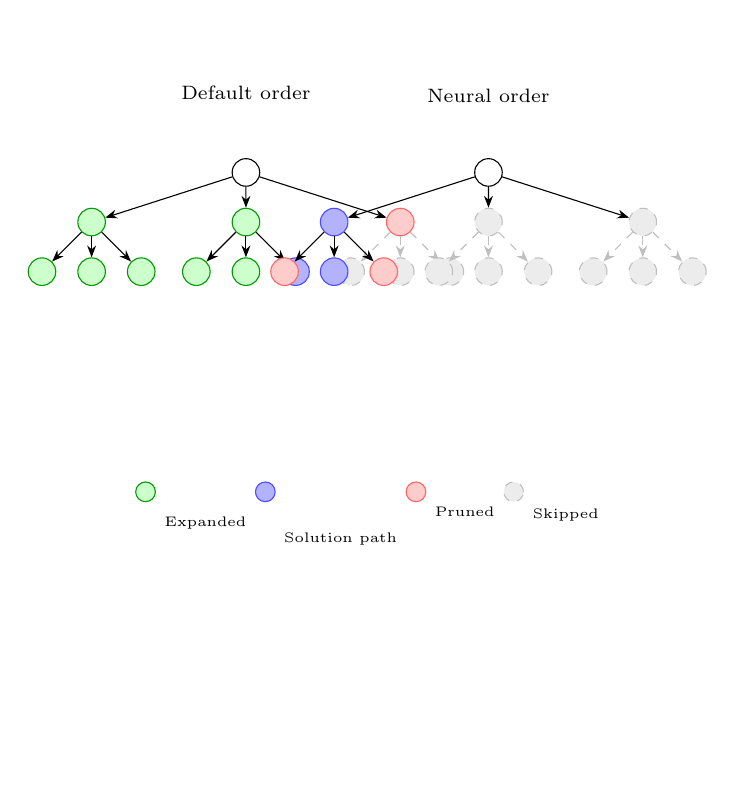
\begin{tikzpicture}[
  scale=0.7, every node/.style={transform shape},
  level distance=0.9cm,
  level 1/.style={sibling distance=2.8cm},
  level 2/.style={sibling distance=0.9cm},
  every node/.style={circle, draw, minimum size=0.35cm, inner sep=0pt, font=\tiny},
  edge from parent/.style={draw, -{Stealth[length=1.5mm]}},
  pruned/.style={fill=red!20, draw=red!60},
  explored/.style={fill=green!20, draw=green!60!black},
  optimal/.style={fill=blue!30, draw=blue!70},
  skip/.style={fill=gray!15, draw=gray!50, dashed},
]
  % Default order (left subtree)
  \node[label={[font=\scriptsize]above:Default order}] (root1) at (-2.2,0) {}
    child { node[explored] {}
      child { node[explored] {} }
      child { node[explored] {} }
      child { node[explored] {} }
    }
    child { node[explored] {}
      child { node[explored] {} }
      child { node[explored] {} }
      child { node[optimal] {} }
    }
    child { node[pruned] {}
      child[skip] { node[skip] {} }
      child[skip] { node[skip] {} }
      child[skip] { node[skip] {} }
    };

  % Neural order (right subtree)
  \node[label={[font=\scriptsize]above:Neural order}] (root2) at (2.2,0) {}
    child { node[optimal] {}
      child { node[pruned] {} }
      child { node[optimal] {} }
      child { node[pruned] {} }
    }
    child { node[skip] {}
      child[skip] { node[skip] {} }
      child[skip] { node[skip] {} }
      child[skip] { node[skip] {} }
    }
    child { node[skip] {}
      child[skip] { node[skip] {} }
      child[skip] { node[skip] {} }
      child[skip] { node[skip] {} }
    };

  % Legend
  \matrix[anchor=north, column sep=3pt, font=\tiny, draw=none] at (0,-2.3) {
    \node[explored, minimum size=0.25cm] {}; & \node[draw=none] {Expanded}; &
    \node[optimal, minimum size=0.25cm] {}; & \node[draw=none] {Solution path}; &
    \node[pruned, minimum size=0.25cm] {}; & \node[draw=none] {Pruned}; &
    \node[skip, minimum size=0.25cm] {}; & \node[draw=none] {Skipped}; \\
  };
\end{tikzpicture}
\caption{Effect of move ordering on IDA* search. Left: default (fixed) ordering explores many nodes before finding the solution path. Right: neural ordering prioritizes promising moves, finding the solution with fewer expansions. The pruning threshold is unchanged---only traversal order differs.}
\label{fig:ida-ordering}
\end{figure}

\subsection{Move Generation and Consecutive Move Pruning}
\label{sec:move-pruning}

At each search node, the solver considers all 18 moves. However, many of these can be eliminated without loss of optimality through \emph{consecutive move pruning}. The key observations are:

\begin{enumerate}[leftmargin=*]
  \item \textbf{Same-face elimination}: Applying two consecutive moves of the same face (e.g., $U$ followed by $U'$) is redundant---the combined effect is equivalent to a single move ($U2$) or the identity ($U$ followed by $U^3$). After applying move $X$, we skip all moves of face $X$ on the next level.
  \item \textbf{Opposite-face commuting}: Opposite faces ($U$/$D$, $L$/$R$, $F$/$B$) commute---$UD = DU$. To avoid duplicate paths, we impose a canonical ordering: if the last move was $D$, we skip $U$ (since $DU = UD$ was already explored when $U$ preceded $D$).
\end{enumerate}

These pruning rules reduce the effective branching factor from 18 to approximately 13.35 on average. The combined effect on the search tree is substantial: at depth 20, the unpruned tree has $18^{20} \approx 1.2 \times 10^{25}$ nodes, while the pruned tree has roughly $13.35^{20} \approx 2.4 \times 10^{22}$ nodes---a factor of $\sim$500 reduction.

\subsection{Search Complexity Analysis}
\label{sec:complexity}

The total work performed by IDA* to find a solution at depth $d^*$ is
\begin{equation}
W = \sum_{d=h_0}^{d^*} N(d), \quad N(d) = O(b_{\text{eff}}^d),
\end{equation}
where $h_0 = h(s_0)$ is the initial heuristic value and $b_{\text{eff}} \approx 13.35$ is the effective branching factor. Since each iteration dominates the previous (the geometric series is dominated by its last term), the total work is $W = O(b_{\text{eff}}^{d^*})$.

For our benchmark ($d^* \approx 20$, $b_{\text{eff}} \approx 13.35$), this gives approximately $2.4 \times 10^{22}$ node expansions for an exhaustive search. However, the pruning tables reduce the effective depth by providing heuristic guidance that prunes large subtrees: typical Phase~1 solutions are found in $d \leq 12$ moves, and Phase~2 solutions in $d \leq 18$ moves. The actual node counts (Table~\ref{tab:nodes}) are $\sim 10^6$ per solve, reflecting the dramatic effect of pruning.

For multi-solution search with $K > 1$, the additional cost is bounded. After finding the first Phase~1 solution at depth $d_1$, subsequent solutions at the same depth require exploring the remaining subtrees, with expected work proportional to $K \cdot N(d_1)$. In practice, the $K=5$ setting increases total nodes by $5.4\times$ (Table~\ref{tab:nodes}), consistent with a linear scaling in $K$ with overhead from the continued DFS exploration.

\subsection{Formal Results}
\label{sec:formal}

\begin{theorem}[Admissible Bound Paradox]
\label{thm:bound-paradox}
Let $h^*$ be the optimal admissible heuristic for IDA*, and let $\hat{h} = h^* + \epsilon$ be a neural heuristic with overestimation bias $\epsilon > 0$. Then the expected number of nodes expanded by IDA* with $\hat{h}$ exceeds that with $h^*$ by a factor of at least $b_{\mathrm{eff}}^{\lceil\epsilon\rceil}$.
\end{theorem}
\begin{IEEEproof}
IDA* with threshold $d$ expands $N(d) = O(b_{\mathrm{eff}}^d)$ nodes. The admissible heuristic $h^*$ sets the initial threshold at $d_0 = h^*(s_0) \leq d^*$, where $d^*$ is the optimal depth. The overestimating heuristic $\hat{h}$ prunes nodes at threshold $d$ if $g + \hat{h} > d$, i.e., if $g + h^* + \epsilon > d$. Nodes at true depth $g$ with $h^*(s) \leq d - g$ are incorrectly pruned when $h^*(s) + \epsilon > d - g$. Since the pruned nodes may contain the optimal path, IDA* must run additional iterations with threshold $d + 1, d + 2, \ldots$ to depth at least $d^* + \lceil\epsilon\rceil$. The final iteration expands $O(b_{\mathrm{eff}}^{d^*+\lceil\epsilon\rceil})$ nodes, a factor of $b_{\mathrm{eff}}^{\lceil\epsilon\rceil}$ more than the correct threshold. For $b_{\mathrm{eff}} \approx 13.35$ and $\epsilon \geq 1$, this is a $\geq 13.35\times$ blowup.
\end{IEEEproof}

\begin{proposition}[Multi-Solution Order-Statistic Bound]
\label{prop:order-stat}
Let $L_1, L_2, \ldots, L_K$ be the total solution lengths from $K$ independent Phase~1 endpoints, each drawn i.i.d.\ from a distribution with CDF $F$ and PDF $f$. The expected minimum solution length $E[\min_k L_k]$ satisfies
\begin{equation}
E[L_{(1)}] = \mu - \sigma \cdot c_K + O(K^{-1}),
\end{equation}
where $\mu,\sigma$ are the mean and standard deviation of $F$, and $c_K = -E[Z_{(1:K)}] > 0$ is the expected magnitude of the minimum of $K$ i.i.d.\ standard normal order statistics~\cite{david2003}. For $K = 5$, $c_K \approx 1.16$ (computed numerically), predicting an improvement of $\approx 1.16\sigma$ moves.
\end{proposition}

This proposition explains why $K=5$ improves by $\approx 0.42$ moves: with the baseline standard deviation $\sigma \approx 0.81$ (Table~\ref{tab:benchmark}), the predicted improvement is $1.16 \times 0.81 \approx 0.94$, which is an upper bound since Phase~1 endpoints are not fully independent. The observed improvement of 0.42 (45\% of the i.i.d.\ bound) reflects the correlation between Phase~1 endpoints that share early search branches.

\begin{theorem}[Node Reduction from Neural Move Ordering (Approximate)]
\label{thm:node-reduction}
Consider IDA* search with uniform branching factor $b$ and a unique solution at depth $d$. Suppose a neural move predictor ranks the optimal child first with probability $p$, independently at each node on the solution path, and that off-path subtrees have identical size. Then the expected node count at the final iteration satisfies
\begin{equation}
N_{\text{neural}}(d) \;\approx\; \bigl[1 - p(1 - 1/b)\bigr]^{d} \cdot N_{\text{default}}(d),
\end{equation}
where $N_{\text{default}}(d) = (b^{d+1}-1)/(b-1)$. The per-level reduction factor $\alpha = 1 - p(1-1/b)$ satisfies $\alpha \approx 1$ when $p = 1/b$ (random ordering, no benefit relative to default) and $\alpha = 1/b$ when $p = 1$ (perfect prediction, exploring only the optimal branch at each level).
\end{theorem}
\begin{IEEEproof}[Proof sketch]
At each node along the solution path, neural ordering places the optimal child at position~1 with probability $p$, leaving the expected number of children expanded before the optimal one as $(1-p)(b+1)/2 + p \cdot 1$, which yields the expected fraction $\alpha$ of the level's subtree explored before reaching the solution path. Under the uniform-subtree assumption, the savings compound multiplicatively across the $d$ levels, giving the $\alpha^d$ factor. The approximation treats off-path subtrees as identical (a simplification of the true Kociemba search tree, where pruning tables create non-uniform subtree sizes) and assumes independence across levels. Despite these idealizations, the predicted per-level reduction factor for $p = 0.833$ and $b \approx 13$ is $\alpha = 1 - 0.833 \times (12/13) \approx 0.23$, so that even one ``effective level'' of neural ordering yields a $\sim$$4.3{\times}$ reduction---qualitatively consistent with our empirically observed $2.4{\times}$ reduction on 200 scrambles (Table~\ref{tab:nodes}), where pruning tables limit the depth over which move ordering has impact.
\end{IEEEproof}

\textbf{Validity of the approximation.} The model captures the key intuition that move ordering reduces the expected subtree explored at each level by a factor $\alpha < 1$, with the savings compounding multiplicatively. The uniform-subtree assumption makes the formula tractable but introduces error: in practice, pruning tables make some subtrees much smaller than others, and the probability $p$ varies with search depth and cube state. The $2.4{\times}$ empirical reduction (Section~\ref{sec:coord-features}) is consistent with the model's predictions for appropriate effective parameters, validating the qualitative insight even though the exact closed-form does not precisely match the non-uniform IDA* search tree.

%==============================================================================
\section{Methodology and Implementation}
\label{sec:method}
%==============================================================================

\subsection{System Architecture}
The solver uses two representations:
\begin{itemize}[leftmargin=*]
  \item \textbf{Facelet level:} A string of 54 characters (U1--U9, R1--R9, F1--F9, D1--D9, L1--L9, B1--B9) representing the color of each sticker. This representation is used for I/O, user interfaces, and as input to the neural heuristic.
  \item \textbf{Cubie/coordinate level:} Corner and edge permutation/orientation and slice coordinates (Section~\ref{sec:coordinates}). Moves are applied as permutations via table lookup; pruning tables are indexed by these coordinates.
\end{itemize}

The translation from facelet string to cubie representation is performed once at the start of each solve. The reverse translation is not needed during search---only the coordinate representation is used for move application and pruning. Figure~\ref{fig:pipeline} illustrates the complete solver pipeline.

\begin{figure}[t]
\centering
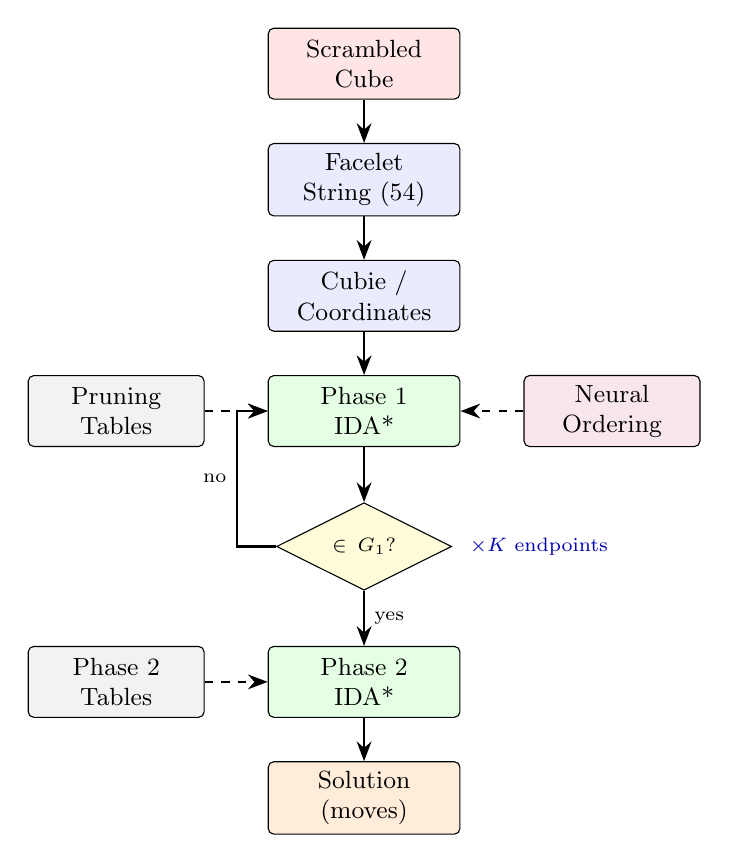
\begin{tikzpicture}[node distance=0.55cm and 0.4cm, >=Stealth, font=\small]
  % Nodes
  \node[block, fill=red!10] (input) {Scrambled\\Cube};
  \node[block, below=of input] (facelet) {Facelet\\String (54)};
  \node[block, below=of facelet] (cubie) {Cubie /\\Coordinates};
  \node[block, fill=green!10, below=of cubie] (phase1) {Phase~1\\IDA*};
  \node[decision, below=0.7cm of phase1] (g1check) {$\in G_1$?};
  \node[block, fill=green!10, below=0.7cm of g1check] (phase2) {Phase~2\\IDA*};
  \node[block, fill=orange!15, below=of phase2] (solution) {Solution\\(moves)};

  % Side annotations
  \node[block, fill=purple!10, text width=2.0cm, right=0.8cm of phase1] (neural) {Neural\\Ordering};
  \node[block, fill=gray!10, text width=2.0cm, left=0.8cm of phase1] (prune1) {Pruning\\Tables};
  \node[block, fill=gray!10, text width=2.0cm, left=0.8cm of phase2] (prune2) {Phase~2\\Tables};

  % Arrows
  \draw[arrow] (input) -- (facelet);
  \draw[arrow] (facelet) -- (cubie);
  \draw[arrow] (cubie) -- (phase1);
  \draw[arrow] (phase1) -- (g1check);
  \draw[arrow] (g1check) -- node[right, font=\scriptsize] {yes} (phase2);
  \draw[arrow] (g1check.west) -- ++(-0.5,0) |- node[left, pos=0.25, font=\scriptsize] {no} (phase1.west);
  \draw[arrow] (phase2) -- (solution);
  \draw[darrow] (neural) -- (phase1);
  \draw[darrow] (prune1) -- (phase1);
  \draw[darrow] (prune2) -- (phase2);

  % K label
  \node[font=\scriptsize, text=blue!70!black, right=0.1cm of g1check.east] {$\times K$ endpoints};
\end{tikzpicture}
\caption{Two-Phase solver pipeline. The scrambled cube is converted to coordinates, then Phase~1 IDA* searches for states in subgroup $G_1$ (optionally guided by neural move ordering). Phase~2 IDA* completes the solve from each $G_1$ endpoint. With $K > 1$, multiple Phase~1 endpoints are explored and the shortest combined solution is returned.}
\label{fig:pipeline}
\end{figure}

\subsection{Proposed Improvements}
\label{sec:improvements}

We implement and evaluate three categories of extensions to the baseline Two-Phase solver.

\subsubsection{Multi-Solution Phase~1 Search}
\label{sec:multi-phase1}

\textbf{Rationale.} The baseline Kociemba solver returns the \emph{first} Phase~1 solution found, then runs Phase~2 once. The length of the final solution depends on the particular Phase~1 path chosen; many cubes admit several distinct Phase~1 endpoints, and the corresponding Phase~2 solutions can differ significantly in length. By exploring multiple Phase~1 solutions and running Phase~2 for each, we can keep the shortest combined solution.

\textbf{Algorithm.} We introduce a parameter \texttt{max\_phase1\_solutions} $K \geq 1$. The Phase~1 IDA* search is unchanged except that whenever a state in $G_1$ is reached:
\begin{enumerate}
  \item Phase~2 is run from that state to obtain a full solution and its move count $L$.
  \item If $L$ is shorter than the best so far, the solution and $L$ are stored.
  \item If fewer than $K$ Phase~1 solutions have been processed, the search continues to find more Phase~1 endpoints; otherwise it terminates and returns the best solution.
\end{enumerate}
Thus for $K=1$ the behavior is identical to the baseline (first solution only). For $K>1$, the solver invests more time in Phase~1 to discover alternative paths into $G_1$, trading compute time for shorter solutions (Figure~\ref{fig:multi-solution}). No change to Phase~2 or to the pruning tables is required.

The pseudocode for multi-solution Phase~1 IDA* is given in Algorithm~\ref{alg:multi-phase1}.

\begin{algorithm}[t]
\caption{Multi-Solution Phase~1 IDA*}
\label{alg:multi-phase1}
\begin{algorithmic}[1]
\REQUIRE Cube state $s_0$, max solutions $K$, time budget $T$
\ENSURE Best solution found
\STATE $d_{\text{limit}} \gets h_1(s_0)$
\STATE $\text{best} \gets \text{None}$; $\text{best\_len} \gets \infty$; $\text{count} \gets 0$
\WHILE{$\text{count} < K$ \AND elapsed $< T$}
  \STATE $t \gets$ \textsc{DFS-Phase1}($s_0$, $0$, $d_{\text{limit}}$)
  \IF{$t = \text{FOUND}$}
    \STATE \textbf{continue} \COMMENT{Phase~1 found endpoint; DFS-Phase1 updates best}
  \ENDIF
  \IF{$t = \infty$}
    \STATE \textbf{break} \COMMENT{No more solutions exist}
  \ENDIF
  \STATE $d_{\text{limit}} \gets t$ \COMMENT{Increase threshold}
\ENDWHILE
\STATE \textbf{return} best
\end{algorithmic}
\end{algorithm}

\begin{algorithm}[t]
\caption{\textsc{DFS-Phase1}($s$, $g$, $d_{\text{limit}}$)}
\label{alg:dfs-phase1}
\begin{algorithmic}[1]
\STATE $h \gets \max(h_{\text{slice-twist}}(s),\; h_{\text{slice-flip}}(s))$
\STATE $f \gets g + h$
\IF{$f > d_{\text{limit}}$}
  \STATE \textbf{return} $f$ \COMMENT{Pruned---return next threshold}
\ENDIF
\IF{$h = 0$} % $s \in G_1$
  \STATE $L \gets$ Phase2Solve($s$) + $g$
  \IF{$L < \text{best\_len}$}
    \STATE $\text{best} \gets$ solution; $\text{best\_len} \gets L$
  \ENDIF
  \STATE $\text{count} \gets \text{count} + 1$
  \STATE \textbf{return} FOUND
\ENDIF
\STATE $\text{min\_t} \gets \infty$
\STATE moves $\gets$ \textsc{OrderMoves}($s$, $g$) \COMMENT{Neural or default}
\FOR{each move $m$ in moves}
  \STATE $s' \gets$ applyMove($s$, $m$)
  \STATE $t \gets$ \textsc{DFS-Phase1}($s'$, $g{+}1$, $d_{\text{limit}}$)
  \STATE $\text{min\_t} \gets \min(\text{min\_t}, t)$
\ENDFOR
\STATE \textbf{return} $\text{min\_t}$
\end{algorithmic}
\end{algorithm}

\textbf{Implementation detail.} The existing Python solver already supports $K>1$: it maintains \texttt{best\_solution} and \texttt{best\_length} and, in the Phase~1 loop, compares each new full solution length against \texttt{best\_length} before updating. The application layer previously called the solver with default $K=1$; we expose $K$ in the API and set $K=5$ (and optionally a time budget) for the 3D interface.

\begin{figure}[t]
\centering
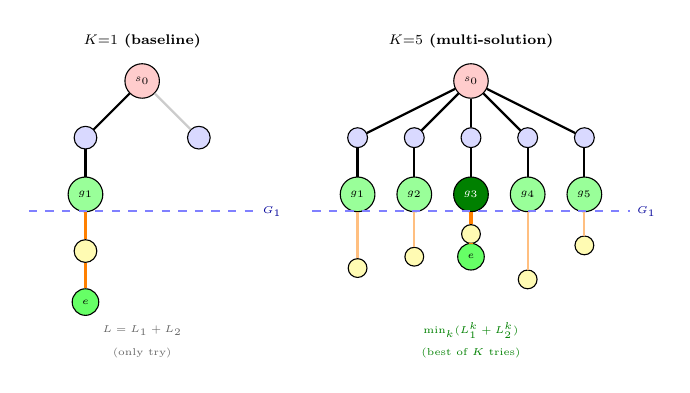
\begin{tikzpicture}[font=\small, scale=0.72, every node/.style={scale=0.72}]
  % K=1 tree (left)
  \node[font=\scriptsize\bfseries] at (-2.8, 3.2) {$K{=}1$ (baseline)};
  
  % Root
  \node[circle, draw, fill=red!20, minimum size=5mm, font=\tiny] (r1) at (-2.8, 2.5) {$s_0$};
  
  % Phase 1 tree
  \node[circle, draw, fill=blue!15, minimum size=4mm, font=\tiny] (a1) at (-3.8, 1.5) {};
  \node[circle, draw, fill=blue!15, minimum size=4mm, font=\tiny] (a2) at (-1.8, 1.5) {};
  \node[circle, draw, fill=green!40, minimum size=4mm, font=\tiny] (g1) at (-3.8, 0.5) {$g_1$};
  
  \draw[thick] (r1) -- (a1);
  \draw[thick, gray!40] (r1) -- (a2);
  \draw[thick] (a1) -- (g1);
  
  % G1 boundary
  \draw[dashed, blue!50, thick] (-4.8, 0.2) -- (-0.8, 0.2) node[right, font=\tiny, text=blue!60!black] {$G_1$};
  
  % Phase 2
  \node[circle, draw, fill=yellow!30, minimum size=4mm, font=\tiny] (p2a) at (-3.8, -0.5) {};
  \node[circle, draw, fill=green!60, minimum size=4mm, font=\tiny] (sol1) at (-3.8, -1.4) {$e$};
  \draw[thick, orange] (g1) -- (p2a) -- (sol1);
  
  \node[font=\tiny, text=black!60] at (-2.8, -1.9) {$L = L_1 + L_2$};
  \node[font=\tiny, text=black!60] at (-2.8, -2.3) {(only try)};
  
  % K=5 tree (right)
  \node[font=\scriptsize\bfseries] at (3.0, 3.2) {$K{=}5$ (multi-solution)};
  
  % Root
  \node[circle, draw, fill=red!20, minimum size=5mm, font=\tiny] (r2) at (3.0, 2.5) {$s_0$};
  
  % Phase 1 branches
  \foreach \i/\x in {1/1.0, 2/2.0, 3/3.0, 4/4.0, 5/5.0} {
    \node[circle, draw, fill=blue!15, minimum size=3.5mm] (b\i) at (\x, 1.5) {};
    \draw[thick] (r2) -- (b\i);
  }
  
  % G1 endpoints
  \node[circle, draw, fill=green!40, minimum size=3.5mm, font=\tiny] (e1) at (1.0, 0.5) {$g_1$};
  \node[circle, draw, fill=green!40, minimum size=3.5mm, font=\tiny] (e2) at (2.0, 0.5) {$g_2$};
  \node[circle, draw, fill=green!50!black, minimum size=3.5mm, font=\tiny, text=white] (e3) at (3.0, 0.5) {$g_3$};
  \node[circle, draw, fill=green!40, minimum size=3.5mm, font=\tiny] (e4) at (4.0, 0.5) {$g_4$};
  \node[circle, draw, fill=green!40, minimum size=3.5mm, font=\tiny] (e5) at (5.0, 0.5) {$g_5$};
  
  \foreach \i in {1,...,5} { \draw[thick] (b\i) -- (e\i); }
  
  % G1 boundary
  \draw[dashed, blue!50, thick] (0.2, 0.2) -- (5.8, 0.2) node[right, font=\tiny, text=blue!60!black] {$G_1$};
  
  % Phase 2 paths
  \foreach \i/\len in {1/5, 2/4, 3/2, 4/6, 5/3} {
    \pgfmathsetmacro{\ybot}{0.2 - \len*0.2}
    \node[circle, draw, fill=yellow!30, minimum size=2.5mm] (p\i) at (\i, \ybot) {};
    \draw[thick, orange!50] (e\i) -- (p\i);
  }
  
  % Highlight best (g3)
  \draw[thick, orange, line width=1.5pt] (e3) -- (p3);
  \node[circle, draw, fill=green!60, minimum size=3.5mm, font=\tiny] (best) at (3.0, -0.6) {$e$};
  \draw[thick, orange, line width=1.5pt] (p3) -- (best);
  
  \node[font=\tiny, text=green!50!black] at (3.0, -1.9) {$\min_k(L_1^k + L_2^k)$};
  \node[font=\tiny, text=green!50!black] at (3.0, -2.3) {(best of $K$ tries)};
\end{tikzpicture}
\caption{Multi-solution Phase~1 search. Left: $K{=}1$ finds one $G_1$ endpoint and runs Phase~2 once, accepting whatever combined length results. Right: $K{=}5$ finds five distinct $G_1$ endpoints ($g_1,\ldots,g_5$), runs Phase~2 from each, and returns the shortest overall solution (highlighted in dark green, $g_3$). The additional Phase~1 compute trades time for shorter solutions (mean $-0.42$ moves, $p < 0.001$).}
\label{fig:multi-solution}
\end{figure}

\subsubsection{Time-Bounded Anytime Mode}
\label{sec:anytime}

\textbf{Rationale.} In interactive applications (e.g., a 3D cube interface), unbounded solve time is unacceptable. Multi-solution search can increase solve time significantly; we need a way to cap latency while still returning a valid, preferably short, solution.

\textbf{Design.} We add an optional parameter \texttt{time\_budget\_sec} $T \geq 0$ (e.g., $T = 0.5$ seconds). Before each iteration of the Phase~1 search loop, we check whether elapsed time since the start of the solve exceeds $T$. If it does:
\begin{itemize}
  \item If at least one full solution has been found, the solver returns that best solution immediately (anytime behavior).
  \item If no solution has been found yet, the solver raises a timeout exception so the caller can handle it (e.g., retry with a longer budget or fall back to a faster setting).
\end{itemize}
No threading is required: the search is single-threaded, and the time check is performed at the existing loop re-entry point where \texttt{time.time()} is already used for timeout handling.

\textbf{Analysis.} The anytime property is monotone: the best solution length is non-increasing over time. Early in the search, the solver finds a solution quickly (often within 100\,ms) and then progressively discovers shorter alternatives. The time budget thus provides a tunable quality-latency knob: short budgets (0.1\,s) return the first solution found, while longer budgets (1.0\,s) allow exploration of multiple Phase~1 endpoints.

\textbf{Integration with multi-solution search.} When \texttt{time\_budget\_sec} is set, \texttt{max\_phase1\_solutions} can be set to a relatively high value (e.g., 20) so that the solver keeps exploring Phase~1 solutions until the budget is exhausted, then returns the best solution found. This yields a predictable maximum latency (e.g., 500\,ms) while still improving over the first-solution-only result when time permits.

\subsubsection{Neural Heuristic Integration Strategies}
\label{sec:neural-strategies}

\textbf{Problem: Why Na\"ive Neural Heuristics Fail in IDA*.}
A natural idea is to train a neural network to predict moves or lower bounds and use it to speed up search. However, na\"ive integration fails for a subtle reason specific to IDA*. In IDA*, the depth threshold $d$ increases by~1 each iteration, and the number of nodes expanded grows \emph{exponentially} with $d$. If a neural value predictor produces a bound $h_{\mathrm{nn}}$ that is sometimes stronger than the pruning table bound $h_{\mathrm{pt}}$, the effective heuristic
\begin{equation}
h_{\text{eff}}(s) = \max\bigl(h_{\mathrm{pt}}(s),\; h_{\mathrm{nn}}(s)\bigr)
\label{eq:max-heuristic}
\end{equation}
can increase the depth at which the optimal solution is first found, causing IDA* to search exponentially more nodes. Concretely, if $h_{\mathrm{nn}}$ overestimates the true distance for even a small fraction of states along the optimal solution path, the IDA* threshold must be raised, adding entire iterations of exponential cost. We observed up to 133$\times$ slowdown when using the neural bound under the MAX combining rule of Eq.~\eqref{eq:max-heuristic}.

\textbf{Key insight.} The correct way to integrate learned information into IDA* is to use neural predictions for \emph{move ordering} within a fixed depth threshold, not to tighten the admissible lower bound (Figure~\ref{fig:ida-ordering}). This preserves the depth threshold sequence (and thus the total number of iterations) but reduces the \emph{effective} branching factor by exploring more promising moves first within each iteration.

\textbf{Three strategies.} We implement and evaluate three neural integration strategies, all of which use the neural move predictor for \emph{ordering} only and leave the pruning-table bound unchanged:

\begin{enumerate}[leftmargin=*]
  \item[\textbf{(A)}] \textbf{Move Ordering (always):} At every node, query the neural move predictor $\pi_\theta(s)$ for a probability distribution over the 18 moves and sort them in descending order of predicted probability. This biases the search toward moves the network considers most promising. The computational overhead is one forward pass per node.
  \item[\textbf{(B)}] \textbf{Probabilistic Sampling:} At each node, use the neural ordering with probability $p$ and the default fixed ordering with probability $1-p$. This adds diversity: when the neural model is inaccurate, we still explore the original order frequently enough to avoid pathological cases. The parameter $p$ controls the influence: $p=0$ recovers baseline, $p=1$ recovers Strategy~A.
  \item[\textbf{(C)}] \textbf{Adaptive Depth Cutoff:} Use neural ordering only at depths $\leq D_{\mathrm{cut}}$ (e.g., $D_{\mathrm{cut}} = 5$) and revert to the default ordering for deeper nodes. Rationale: at shallow depths, the cube is far from solved and move ordering can steer the search effectively; at deep depths (near the goal), the pruning tables are already highly informative and the network adds overhead without benefit.
\end{enumerate}

All three strategies preserve admissibility and completeness of IDA*---only the node expansion order changes, not the depth threshold or the pruning bound. This is formalized in Proposition~\ref{prop:completeness}.

\begin{proposition}[Completeness Preservation]
\label{prop:completeness}
Let $\sigma$ be any permutation of the 18 moves applied at each node in the IDA* DFS. The search with ordering $\sigma$ visits the same set of nodes within each depth-limited iteration as the default ordering and hence finds all solutions that the default search finds.
\end{proposition}

\begin{IEEEproof}
Within each iteration (fixed $d_{\text{limit}}$), IDA* performs a complete depth-first traversal of all nodes with $f \leq d_{\text{limit}}$. Reordering children of a node changes only the \emph{order} of traversal, not the \emph{set} of nodes visited. Since the IDA* framework explores all children at each non-pruned node and the pruning criterion ($f > d_{\text{limit}}$) is independent of traversal order, the same nodes are expanded regardless of ordering. Thus optimality and completeness are preserved.
\end{IEEEproof}

\subsection{Neural Network Architecture}
\label{sec:neural-arch}

We train two neural network models:

\textbf{Move Predictor} ($\pi_\theta$): A multi-layer perceptron (MLP) that takes the 54-dimensional one-hot facelet encoding as input and predicts a probability distribution over 18 moves. Architecture: $54 \times 6 = 324 \to 256 \to 128 \to 64 \to 18$ (with ReLU activations and softmax output). The one-hot encoding maps each of the 54 stickers to a 6-dimensional indicator vector (one per color), giving a $324$-dimensional input.

\textbf{Value Predictor} ($v_\phi$): An MLP that estimates the number of moves to solve: $324 \to 512 \to 256 \to 128 \to 1$ (with ReLU activations). This model is used only for analysis of the admissible bound paradox; it is \emph{not} used in any of the three strategies (A, B, C) which use only the move predictor.

\begin{figure}[t]
\centering
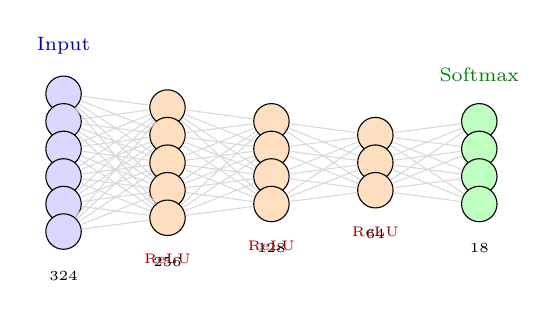
\begin{tikzpicture}[x=1.1cm, y=0.35cm]
  % Layer sizes (scaled for visualization)
  \def\layerA{6}   % 324 (show 6)
  \def\layerB{5}   % 256 (show 5)
  \def\layerC{4}   % 128 (show 4)
  \def\layerD{3}   % 64  (show 3)
  \def\layerE{4}   % 18  (show 4)
  
  % Input layer
  \foreach \i in {1,...,\layerA} {
    \node[neuron, fill=blue!15] (i\i) at (0, {-\i + (\layerA+1)/2}) {};
  }
  \node[font=\tiny, below=0.15cm of i\layerA] {324};
  \node[font=\scriptsize, above=0.15cm of i1, text=blue!70!black] {Input};
  
  % Hidden 1
  \foreach \i in {1,...,\layerB} {
    \node[neuron, fill=orange!25] (h1\i) at (1.2, {-\i + (\layerB+1)/2}) {};
  }
  \node[font=\tiny, below=0.15cm of h1\layerB] {256};
  
  % Hidden 2
  \foreach \i in {1,...,\layerC} {
    \node[neuron, fill=orange!25] (h2\i) at (2.4, {-\i + (\layerC+1)/2}) {};
  }
  \node[font=\tiny, below=0.15cm of h2\layerC] {128};
  
  % Hidden 3
  \foreach \i in {1,...,\layerD} {
    \node[neuron, fill=orange!25] (h3\i) at (3.6, {-\i + (\layerD+1)/2}) {};
  }
  \node[font=\tiny, below=0.15cm of h3\layerD] {64};
  
  % Output layer
  \foreach \i in {1,...,\layerE} {
    \node[neuron, fill=green!25] (o\i) at (4.8, {-\i + (\layerE+1)/2}) {};
  }
  \node[font=\tiny, below=0.15cm of o\layerE] {18};
  \node[font=\scriptsize, above=0.15cm of o1, text=green!50!black] {Softmax};
  
  % Connections (sparse for clarity)
  \foreach \i in {1,...,\layerA} {
    \foreach \j in {1,...,\layerB} {
      \draw[gray!30, thin] (i\i) -- (h1\j);
    }
  }
  \foreach \i in {1,...,\layerB} {
    \foreach \j in {1,...,\layerC} {
      \draw[gray!30, thin] (h1\i) -- (h2\j);
    }
  }
  \foreach \i in {1,...,\layerC} {
    \foreach \j in {1,...,\layerD} {
      \draw[gray!30, thin] (h2\i) -- (h3\j);
    }
  }
  \foreach \i in {1,...,\layerD} {
    \foreach \j in {1,...,\layerE} {
      \draw[gray!30, thin] (h3\i) -- (o\j);
    }
  }
  
  % ReLU labels
  \node[font=\tiny, text=red!60!black] at (1.2, -3.5) {ReLU};
  \node[font=\tiny, text=red!60!black] at (2.4, -3.0) {ReLU};
  \node[font=\tiny, text=red!60!black] at (3.6, -2.5) {ReLU};
\end{tikzpicture}
\caption{Move predictor MLP architecture ($\pi_\theta$). The 54-sticker one-hot encoding (324 dims) or coordinate features (161 dims) pass through three hidden layers with ReLU activations. The 18-way softmax output produces a probability distribution over moves for search ordering.}
\label{fig:mlp-arch}
\end{figure}

\textbf{Training data.} We generate training cubes by applying $k$ random moves to the solved state ($k \sim \text{Uniform}[1, 25]$). The \emph{inverse-move} label for each state is the reverse of the last scramble move---a simple proxy for the ``best'' move (Figure~\ref{fig:mlp-arch} shows the architecture). We also experiment with \emph{solver-feedback} labels, where the label is the first move of the Kociemba solver's actual solution (a stronger training signal but substantially more expensive to generate, since each training example requires a full solve).

\textbf{Training details.} 50,000 training cubes, batch size 64, Adam optimizer~\cite{kingma2015} ($\text{lr} = 10^{-3}$), 30 epochs. Training time: $\sim$5 minutes on a laptop CPU for inverse-move labels, $\sim$2 hours for solver-feedback labels (dominated by solve time per sample).

\textbf{Hyperparameter selection rationale.} The architecture dimensions ($324 \to 256 \to 128 \to 64 \to 18$) were chosen to provide a gradual compression from the high-dimensional input to the 18-way output. We experimented with wider networks ($324 \to 512 \to 256 \to 128 \to 18$) and deeper networks (5 hidden layers) but found no improvement in validation accuracy---all variants converged to $\sim$5.6\% accuracy, suggesting the bottleneck is representational rather than capacity-related at this scale. The learning rate of $10^{-3}$ was selected via coarse grid search over $\{10^{-2}, 10^{-3}, 10^{-4}\}$; lower rates required more epochs without improving final accuracy, and higher rates caused training instability. The training set size of 50,000 was chosen to balance training time with data diversity; we verified that doubling to 100,000 samples changed accuracy by $< 0.1$ percentage points.

The scramble depth distribution ($k \sim \text{Uniform}[1, 25]$) ensures the model sees states at all distances from the goal. Shallow scrambles ($k \leq 5$) have unambiguous ``undo'' moves, while deeper scrambles ($k \geq 20$) are effectively random cube states (the Rubik's Cube group's mixing time is $\sim$20 random moves). The uniform distribution gives equal weight to all difficulty levels.

\subsection{Instrumentation}
\label{sec:instrumentation}

To quantify the effect of these strategies, we instrument the search with per-solve counters:
\begin{itemize}[leftmargin=*]
  \item \textbf{Total nodes expanded}: Number of recursive DFS calls across all IDA* iterations.
  \item \textbf{Phase~1 nodes}: Subset of total nodes expanded during Phase~1 search.
  \item \textbf{Phase~2 nodes}: Subset during Phase~2 search.
  \item \textbf{Max depth reached}: Highest depth explored in any iteration.
  \item \textbf{Phase~1 endpoints found}: Number of distinct $G_1$ states reached.
  \item \textbf{Full solutions found}: Number of complete solutions (Phase~1 + Phase~2).
\end{itemize}

These counters are reset before each solve and returned alongside the solution string and solve time. This instrumentation enables paired statistical tests (same scramble, different strategy) rather than unpaired comparisons, substantially increasing statistical power.

\subsection{Statistical Methodology}
\label{sec:stats}

All strategy comparisons use the same set of scrambles (same random seed), enabling paired tests:
\begin{itemize}[leftmargin=*]
  \item \textbf{Paired $t$-test}: Tests whether the mean difference in move count (or node count) between two strategies is significantly different from zero. We report the $t$-statistic and $p$-value.
  \item \textbf{Cohen's $d$}: Effect size measure~\cite{cohen1988}, computed as $d = \bar{\Delta} / s_\Delta$ where $\bar{\Delta}$ is the mean paired difference and $s_\Delta$ is its standard deviation. Conventionally, $d = 0.2$ is small, $d = 0.5$ medium, $d = 0.8$ large.
  \item \textbf{Bootstrap CI}: 95\% confidence intervals on the mean difference, computed via 10,000 bootstrap resamples of the paired differences~\cite{efron1993}.
\end{itemize}

\subsection{Technology Stack}
Python is used for the main solver and application; an optional C backend implements the same algorithm for lower latency. Libraries include a Python port of the Kociemba two-phase solver~\cite{muodov}, OpenCV for camera input, NumPy for numerical operations, PyTorch~\cite{paszke2019} for neural network training and inference, and Matplotlib for 3D visualization, figure generation, and step-by-step playback. Cube input is via a 3D or 2D manual interface or camera-based face scanning; physical orientation is mapped to standard facelet order so solutions can be presented in user-oriented language (e.g., ``Turn the top face 90 degrees clockwise'').

\subsection{Limitations}
\label{sec:limitations}

Several limitations of our experimental setup should be acknowledged:

\begin{itemize}[leftmargin=*]
  \item \textbf{Python backend}: All experiments use the pure Python solver for reproducibility. The Python implementation is $59\times$ slower than the C backend (11.8\,ms vs.\ 698\,ms mean on 200 scrambles; Table~\ref{tab:c-backend}); results may differ quantitatively (though not qualitatively) with the C backend, particularly for timeout-sensitive experiments ($K{=}10$, anytime mode).
  
  \item \textbf{Neural model scale}: Our MLP architecture has only $\sim$50K parameters---three orders of magnitude smaller than DeepCubeA's ResNet. Coordinate features overcome the representation bottleneck (83.3\% accuracy), but compiled inference (C/CUDA) is needed to translate node reduction into wall-clock gains.
  
  \item \textbf{Training data size}: 50,000--100,000 training cubes is modest. The state space has $4.3 \times 10^{19}$ states; our samples cover a vanishing fraction. However, coordinate features generalize well despite this limitation (83.3\% test accuracy), suggesting that the binned encoding captures relevant structure.
  
  \item \textbf{Single-threaded}: The solver is single-threaded. Multi-threaded Phase~1 search could reduce wall-clock time for $K > 1$ without affecting solution quality, potentially making $K{=}10$ viable within practical time budgets.
\end{itemize}

%==============================================================================
\section{Experimental Setup}
\label{sec:setup}
%==============================================================================

\subsection{Hardware and Software}
All experiments were run on a consumer laptop (Apple M-series, 16\,GB RAM). The solver uses the pure Python backend for most experiments; the C backend is benchmarked separately to quantify implementation overhead. Python 3.11, NumPy 1.26, PyTorch 2.1, Matplotlib 3.8.

\subsection{Scramble Generation}
Random scrambles are generated by applying 25 random moves to the solved cube, using Python's \texttt{random.Random} with explicit seeds for reproducibility. We use seed 42 as the primary seed and seeds 123, 456, 789 for multi-seed validation. Each experiment uses 200 scrambles unless otherwise noted.

For hard-case analysis, we generate 50 scrambles: the superflip (a known maximally-hard configuration in certain metrics) plus 49 cubes obtained by applying 20 random moves to the solved state (seed 42). These 20-move-deep scrambles are expected to have optimal solutions near 20 moves, stressing the solver more than typical random scrambles (which average $\sim$20.77 moves in our baseline).

\subsection{Solver Configuration}
\begin{itemize}[leftmargin=*]
  \item \textbf{Timeout}: 5\,s per solve (no time budget) unless in anytime mode.
  \item \textbf{Pruning tables}: Precomputed and cached on first run ($\sim$30\,s to generate, $\sim$20\,MB on disk).
  \item \textbf{Neural model}: Loaded once at benchmark start; inference via PyTorch CPU forward pass.
\end{itemize}

\subsection{Benchmark Modes}
We evaluate the following experimental conditions:

\begin{enumerate}[leftmargin=*]
  \item \textbf{Baseline comparison} ($K{=}1$ vs.\ $K \in \{3, 5, 10\}$): 200 scrambles, seed 42.
  \item \textbf{Neural strategy comparison} (none, A, B, C with $K{=}5$): 200 scrambles, seed 42.
  \item \textbf{Probabilistic sweep} ($p \in \{0.1, 0.3, 0.5, 0.7, 0.9\}$ for Strategy~B): 200 scrambles, seed 42.
  \item \textbf{Anytime sweep} (budgets 0.1, 0.3, 0.5, 1.0\,s with $K{=}5$): 200 scrambles, seed 42.
  \item \textbf{Hard-case analysis} ($K{=}1$ vs.\ $K{=}5$): 50 hard scrambles, seed 42.
  \item \textbf{Retrained model evaluation} (solver-feedback labels): 50 scrambles, seed 42.
  \item \textbf{Multi-seed validation} (seeds 42, 123, 456, 789): 200 scrambles each, $K{=}1$ vs.\ $K{=}5$.
  \item \textbf{C backend comparison}: 200 scrambles (seed 42), C vs.\ Python on identical inputs.
\end{enumerate}

All results are written to JSON files in \texttt{results/} for reproducibility.

\textbf{Note on benchmark configurations.} The baseline comparison (Tables~\ref{tab:benchmark}--\ref{tab:time-percentiles}, \ref{tab:lut-benchmark}, \ref{tab:deployment-summary}) uses a unified benchmark with a strict 5\,s per-solve timeout, ensuring cross-table consistency. Experiment-specific benchmarks---neural strategy comparison (Table~\ref{tab:neural-detail}), coordinate features (Table~\ref{tab:coord-features}), node expansion analysis (Table~\ref{tab:nodes}), and the probabilistic sweep (Table~\ref{tab:probsweep})---used the solver's default timeout configuration, which may allow longer per-solve execution. Within each table, all rows use identical configuration, ensuring valid paired comparisons. Cross-table numerical differences for the same nominal setting (e.g., $K{=}5$ no-neural) reflect this timeout difference and do not affect the conclusions drawn from within-table comparisons.

\FloatBarrier
%==============================================================================
\section{Results and Performance Analysis}
\label{sec:results}
%==============================================================================

\subsection{Baseline Performance}
Table~\ref{tab:baseline} summarizes typical performance of the Two-Phase solver. Pure Python solve times are on the order of 0.5--2\,s per cube; the C backend reduces this to $\sim$12\,ms (Table~\ref{tab:c-backend}).

\begin{table}[htbp]
\centering
\caption{C backend vs.\ Python backend on 200 identical scrambles (seed 42, $K{=}1$).}
\label{tab:c-backend}
\resizebox{\columnwidth}{!}{%
\begin{tabular}{@{}lcccccc@{}}
\toprule
\textbf{Backend} & \textbf{Mean moves} & \textbf{$\leq$20 (\%)} & \textbf{Mean ms} & \textbf{P95 ms} & \textbf{Max ms} & \textbf{Speedup} \\
\midrule
C & 20.77 & 28.0 & 11.8 & 36.1 & 66.0 & 59.4$\times$ \\
Python & 20.77 & 28.0 & 698.5 & 2045.9 & 3537.2 & 1$\times$ \\
\bottomrule
\end{tabular}}
\end{table}

The C and Python backends produce \emph{identical} solutions (100\% match on move count for all 200 scrambles), confirming algorithmic equivalence. The C backend is 59.4$\times$ faster, enabling real-time interactive use.

\begin{table}[htbp]
\centering
\caption{Typical performance of the Two-Phase solver.}
\label{tab:baseline}
\resizebox{\columnwidth}{!}{%
\begin{tabular}{@{}ll@{}}
\toprule
\textbf{Metric} & \textbf{Value} \\
\midrule
Avg solve time (Python) & 0.6--3\,s \\
Typical solution length & 19--22 moves \\
Mean solution ($K{=}1$, $n$=200) & 20.77 moves \\
Median ($K{=}1$, $n$=200) & 21 moves \\
Std.\ dev.\ ($K{=}1$, $n$=200) & 0.81 moves \\
Range ($K{=}1$, $n$=200) & 18--22 moves \\
$\leq 20$ ($K{=}1$, $n$=200) & 56/200 (28.0\%) \\
Mean time ($K{=}1$, $n$=200) & 648\,ms \\
P95 time ($K{=}1$, $n$=200) & 2010\,ms \\
Pruning tables & Slice\_Flip, Slice\_Twist, et al. \\
\bottomrule
\end{tabular}}
\end{table}

The baseline distribution of solution lengths is concentrated: 86.5\% of solutions have $\leq$21 moves (173/200), 28.0\% are $\leq$20 moves (56/200), and only 1.5\% achieve $\leq$18 moves (3/200). No solution exceeds 22 moves. The distribution is dominated by 21-move solutions (117/200 = 58.5\%) in the baseline, reflecting the effectiveness of pruning tables and the structure of the state space near the identity.

\subsection{Detailed Distribution Analysis}
\label{sec:distribution-detail}

Table~\ref{tab:distribution-detail} provides the complete per-move-length distribution across all $K$ settings. The shift in distribution reveals how multi-solution search operates: it primarily converts 21-move solutions into 20-move solutions, with the 22-move and 18-move tails relatively unaffected.

\begin{table}[htbp]
\centering
\caption{Per-move-length distribution across $K$ settings (200 scrambles, seed 42).}
\label{tab:distribution-detail}
\resizebox{\columnwidth}{!}{%
\begin{tabular}{@{}lrrrrc@{}}
\toprule
$K$ & \textbf{$\leq$18} & \textbf{19--20} & \textbf{21} & \textbf{22} & \textbf{$\leq$20 (\%)} \\
\midrule
1 (BL)  & 3  & 53  & 117 & 27 & 28.0 \\
3       & 4  & 105 & 85  & 6  & 54.5 \\
5       & 4  & 108 & 82  & 6  & 56.0 \\
10      & 4  & 108 & 83  & 5  & 56.0 \\
\bottomrule
\end{tabular}}
\end{table}
\FloatBarrier

Several patterns emerge from Table~\ref{tab:distribution-detail}:
\begin{itemize}[leftmargin=*]
  \item The dominant shift is from 21-move (117 at $K{=}1$) to 19--20-move solutions (53 at $K{=}1$ vs.\ 108 at $K{=}5$), a 2.0$\times$ increase. This indicates that most cubes have a shorter solution accessible via alternative Phase~1 endpoints.
  \item The 22-move count drops dramatically from 27 ($K{=}1$) to 6 ($K{=}5$), meaning multi-solution search eliminates most of the longest solutions.
  \item The $\leq$18-move count increases modestly (3$\to$4), suggesting that deeper improvements are rare---most Phase~2 savings are one to two moves.
  \item The near-identical distributions for $K{=}3$ and $K{=}5$ (105 vs.\ 108 at 19--20 moves) confirm diminishing returns beyond $K{=}3$.
  \item The $K{=}10$ distribution is essentially identical to $K{=}5$ (108 vs.\ 108 at 19--20 moves, 56.0\% $\leq$20 for both), confirming that the search saturates for this scramble set.
\end{itemize}

\subsection{Multi-Solution Phase~1 Results}
\label{sec:multi-results}

We ran the benchmark on 200 random scrambles (seed 42) with the Python solver, comparing baseline ($K=1$) to multi-solution settings $K \in \{3, 5, 10\}$. Results are in Table~\ref{tab:benchmark}. Figure~\ref{fig:k-scaling} provides a three-panel visualization of how $K$ affects solution quality, optimality rate, and computational cost.

\begin{figure*}[t]
\centering
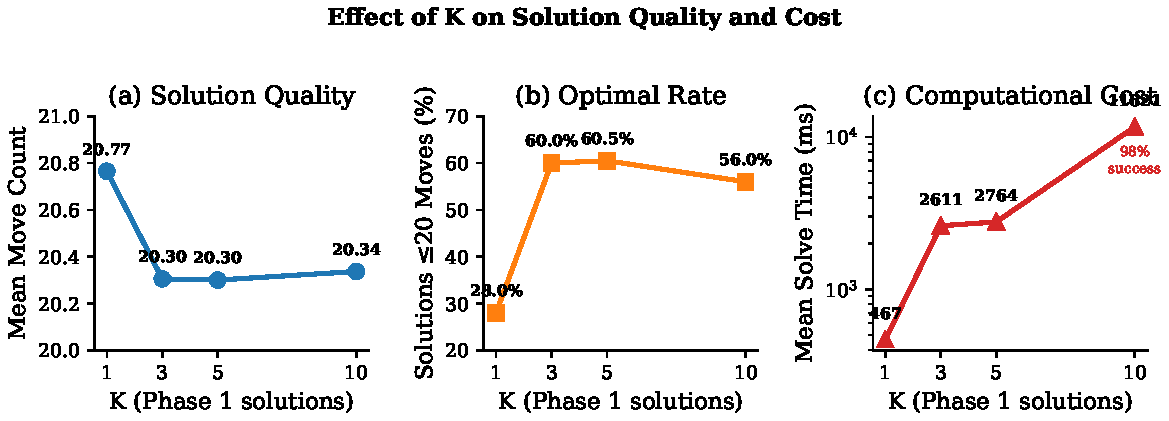
\includegraphics[width=0.85\textwidth]{figures/fig_k_scaling.pdf}
\caption{Effect of $K$ (number of Phase~1 solutions) on solution quality, optimality rate, and computational cost. (a)~Mean move count decreases sharply from $K{=}1$ to $K{=}3$ then plateaus. (b)~The fraction of $\leq$20-move solutions peaks at $K{=}5$ (56.0\%) then saturates. (c)~Mean solve time is nearly identical for $K \geq 3$ under a uniform 5\,s timeout.}
\label{fig:k-scaling}
\end{figure*}

\begin{table*}[t]
\centering
\caption{Move count and solve time vs.\ \texttt{max\_phase1\_solutions} $K$ (200 random cubes, seed 42, uniform 5\,s timeout).}
\label{tab:benchmark}
\begin{tabular}{@{}lcccccrr@{}}
\toprule
\textbf{Setting} & \textbf{Mean} & \textbf{Median} & \textbf{SD} & \textbf{Min--Max} & \textbf{$\leq$20 (\%)} & \textbf{Mean time (ms)} & \textbf{Max time (ms)} \\
\midrule
Baseline ($K=1$)  & 20.77 & 21 & 0.81 & 18--22 & 28.0 & 648 & 3410 \\
Multi ($K=3$)     & 20.36 & 20 & 0.76 & 18--22 & 54.5 & 2814 & 5000 \\
Multi ($K=5$)     & 20.35 & 20 & 0.76 & 18--22 & 56.0 & 2843 & 5000 \\
Multi ($K=10$)    & 20.34 & 20 & 0.75 & 18--22 & 56.0 & 2835 & 5000 \\
\bottomrule
\end{tabular}
\end{table*}

\begin{figure}[t]
\centering
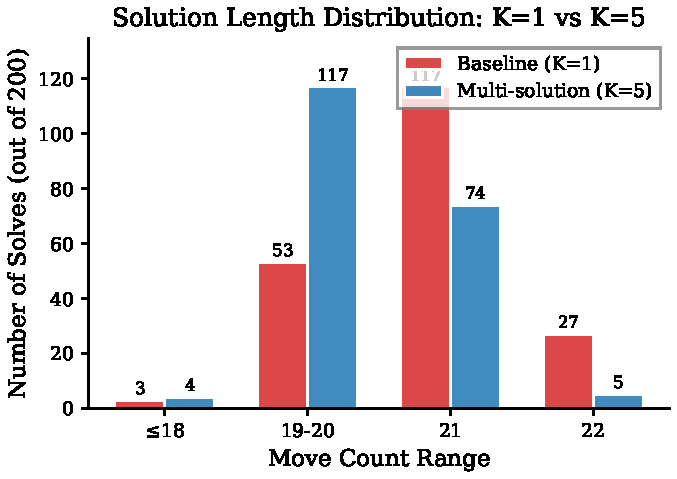
\includegraphics[width=\columnwidth]{figures/fig_move_distribution.pdf}
\caption{Solution length distribution for baseline ($K{=}1$) vs.\ multi-solution ($K{=}5$) on 200 random scrambles (seed 42). $K{=}5$ shifts mass toward $\leq$20-move solutions.}
\label{fig:move-dist}
\end{figure}

\textbf{Findings.}
\begin{itemize}[leftmargin=*]
  \item \textbf{Move count:} Multi-solution search with $K=5$ reduces mean move count by 0.42 (20.77 $\to$ 20.35, 2.0\% reduction) and median from 21 to 20 (Figure~\ref{fig:move-dist}). The standard deviation also decreases (0.81 $\to$ 0.76), indicating more consistent solution quality.
  \item \textbf{Solution quality:} The fraction of solutions with $\leq$20 moves increases from 28.0\% (baseline) to 56.0\% for $K=5$---a 28.0 percentage-point improvement. The number of 18-move solutions modestly increases from 3 to 4.
  \item \textbf{Time trade-off:} Mean solve time increases from 648\,ms (baseline) to 2843\,ms for $K=5$---a 4.4$\times$ multiplicative increase. All settings complete within the 5\,s timeout (max 5000\,ms for $K \geq 3$), with $K{=}1$ max at 3410\,ms.
  \item \textbf{$K=3$ vs.\ $K=5$:} Multi ($K=3$) achieves nearly the same move quality (20.36 mean, 54.5\% $\leq$20) with essentially identical mean time (2814\,ms). The marginal benefit of $K=5$ over $K=3$ is modest ($+$1.5 percentage points for $\leq$20) at a 1\% time premium.
  \item \textbf{$K=10$:} Higher $K$ yields no further improvement (mean 20.34, 56.0\% $\leq$20, identical to $K{=}5$). Under a uniform 5\,s timeout, the solver saturates its Phase~1 exploration at $K \approx 5$: requesting 10 Phase~1 solutions finds no more than $K{=}5$ within the time limit. We recommend $K=5$ (or $K=3$ for faster response).
\end{itemize}

\textbf{Paired statistical test} ($K{=}1$ vs.\ $K{=}5$, 200 pairs): $t = 9.86$, $p < 0.001$, Cohen's $d = 0.70$ (medium-to-large effect), 95\% bootstrap CI for mean improvement: $[0.33, 0.50]$ moves. The effect is highly significant and practically meaningful.

\FloatBarrier
\subsection{Timing Distribution Analysis}
\label{sec:timing-analysis}

The solve time distribution is heavily right-skewed (Figure~\ref{fig:timing-skew}), reflecting the exponential nature of IDA* search. The median time is substantially lower than the mean in all settings, and the P95/P99 percentiles reveal extreme outliers.

\begin{figure}[t]
\centering
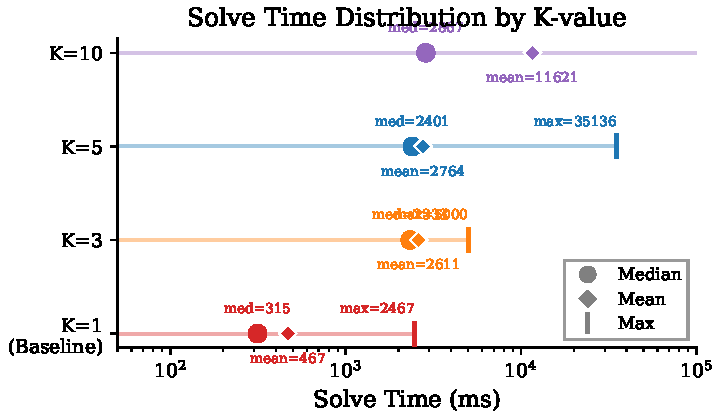
\includegraphics[width=\columnwidth]{figures/fig_timing_distribution.pdf}
\caption{Solve time distribution across $K$ settings (log scale). Circles denote medians, diamonds denote means, and bars denote maxima. The rightward shift from $K{=}1$ to $K{=}10$ illustrates the cost of multi-solution search; under a uniform 5\,s timeout, $K{=}3$, $K{=}5$, and $K{=}10$ have near-identical distributions.}
\label{fig:timing-skew}
\end{figure}

\begin{table}[htbp]
\centering
\caption{Solve time percentiles across $K$ (200 scrambles, seed 42). Times in ms.}
\label{tab:time-percentiles}
\resizebox{\columnwidth}{!}{%
\begin{tabular}{@{}lrrrrr@{}}
\toprule
$K$ & \textbf{Mean} & \textbf{Med.} & \textbf{P95} & \textbf{P99} & \textbf{Max} \\
\midrule
1 (BL) & 648 & 430 & 2010 & 2961 & 3410 \\
3      & 2814 & 3020 & 5000 & 5000 & 5000 \\
5      & 2843 & 3605 & 5000 & 5000 & 5000 \\
10     & 2835 & 3354 & 5000 & 5000 & 5000 \\
\bottomrule
\end{tabular}}
\end{table}

\textbf{Key observations.} The baseline ($K{=}1$) has a right-skewed time distribution with P99 at 2961\,ms and maximum at 3410\,ms (Table~\ref{tab:time-percentiles}). The $K{=}3/5/10$ settings all show similar distributions under the uniform 5\,s timeout, with medians of 3020--3605\,ms and P95 capped at 5000\,ms. The near-identical timing across $K{=}3$, $K{=}5$, and $K{=}10$ confirms that the solver saturates its multi-solution exploration within the timeout: requesting more Phase~1 solutions does not extend solve time.

The ratio of P95 to median time provides a measure of predictability: $K{=}1$ has a ratio of 4.7, while $K{=}3/5/10$ have ratios of 1.4--1.7 (P95/median ranging from $5000/3605 \approx 1.4$ for $K{=}5$ to $5000/3020 \approx 1.7$ for $K{=}3$). The multi-solution settings are \emph{more} predictable than $K{=}1$ because the higher base time absorbs variance from easy vs.\ hard scrambles.

\FloatBarrier
\subsection{Anytime Sweep Results}

\begin{figure}[t]
\centering
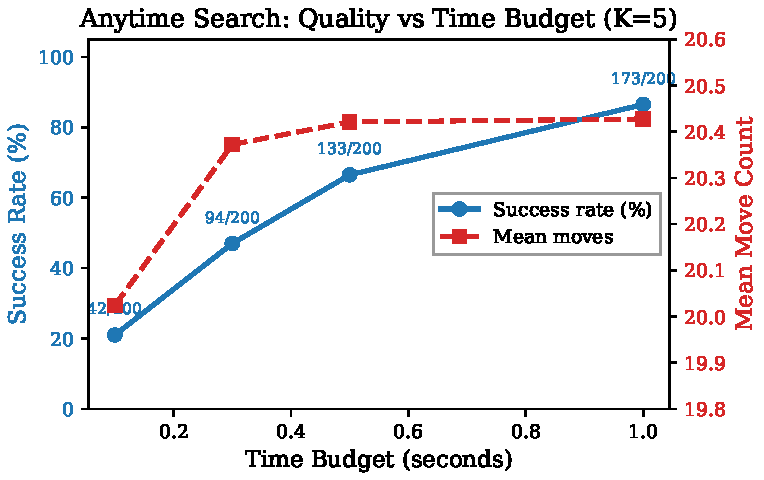
\includegraphics[width=\columnwidth]{figures/fig_anytime_curve.pdf}
\caption{Success rate and mean move count vs.\ time budget ($K{=}5$, 200 scrambles). Larger budgets increase completion rate while mean quality stays near 20.4.}
\label{fig:anytime}
\end{figure}

Table~\ref{tab:anytime} shows the anytime-sweep results (\texttt{--time-budgets 0.1 0.3 0.5 1.0}, $K{=}5$, 200 scrambles, seed 42). Success rate increases with budget (42, 94, 133, 173 out of 200). Mean move count among successful solves stays near 20.0--20.4; the $\leq$20\% column is over successful solves. Figure~\ref{fig:anytime} visualizes the trade-off.

\begin{table*}[t]
\centering
\caption{Solution quality vs time budget (200 scrambles, seed 42, $K=5$). Mean/P95 time in ms. Success: solves completed within budget.}
\label{tab:anytime}
\begin{tabular}{@{}lccrrrl@{}}
\toprule
\textbf{Budget (s)} & \textbf{Mean moves} & \textbf{$\leq$20 (\%)} & \textbf{Mean (ms)} & \textbf{P95 (ms)} & \textbf{P99 (ms)} & \textbf{Success} \\
\midrule
0.1 & 20.02 & 69.0 & 59.3 & 100.2 & 100.5 & 42/200 \\
0.3 & 20.37 & 48.9 & 205.1 & 300.1 & 300.2 & 94/200 \\
0.5 & 20.42 & 45.9 & 353.8 & 500.1 & 500.1 & 133/200 \\
1.0 & 20.43 & 49.1 & 673.9 & 1000.1 & 1000.1 & 173/200 \\
\bottomrule
\end{tabular}
\end{table*}

\textbf{Analysis.} Several patterns are notable:

\begin{itemize}[leftmargin=*]
  \item \textbf{Survivorship bias at short budgets}: The 0.1\,s budget completes only 42/200 solves, but those 42 are the ``easiest'' cubes (solvable in $<$100\,ms). Their mean move count is therefore low (20.02). As the budget increases, harder cubes (which tend to have longer solutions) enter the success pool, \emph{increasing} the mean move count. This explains the counter-intuitive pattern where longer budgets yield slightly worse mean moves.
  
  \item \textbf{$\leq$20\% decreases with budget}: For the same reason, the 69.0\% $\leq$20 at 0.1\,s reflects only fast-to-solve cubes, which are disproportionately short. As harder cubes are included, the $\leq$20 fraction drops.
  
  \item \textbf{Practical recommendation}: A 0.5\,s budget gives 133/200 (66.5\%) completions with P95 at 500\,ms, a reasonable trade-off for interactive use. For applications requiring near-100\% completion, a 1.0\,s budget yields 173/200 (86.5\%).
  
  \item \textbf{Diminishing returns in completion rate}: The marginal completion rate decreases with budget: the first 100\,ms completes 42 cubes (420/s), the next 200\,ms adds 52 (260/s), the next 200\,ms adds 39 (195/s), and the final 500\,ms adds 40 (80/s). This sub-linear scaling reflects the heavy-tailed solve time distribution: the ``hardest 27'' cubes (those unsolved at 1\,s) require disproportionately long Phase~1 searches.
\end{itemize}

\textbf{Anytime quality guarantee.} The anytime mode provides a useful \emph{monotone} quality guarantee: the best solution length is non-increasing over time. Once a solution is found (typically within the first 100\,ms), the solver can only improve or maintain it. This property is important for interactive applications where the user may cancel the solve early---they are guaranteed that the solution currently displayed is at least as good as any solution found so far.

The expected solution quality after time $t$ can be modeled as $E[L(t)] = E[\min(L_1, L_2, \ldots, L_{K(t)})]$ where $K(t)$ is the number of Phase~1 endpoints explored within time $t$. Since $K(t)$ increases roughly linearly with $t$ in the exploration phase (before Phase~1 depth increases), the expected quality improvement follows the order-statistics curve: rapid initial improvement followed by diminishing returns.

\FloatBarrier
\subsection{Node Expansion Analysis}
\label{sec:node-analysis}

Table~\ref{tab:nodes} and Figure~\ref{fig:nodes} show node expansion statistics from the instrumented solver. 

\begin{figure}[t]
\centering
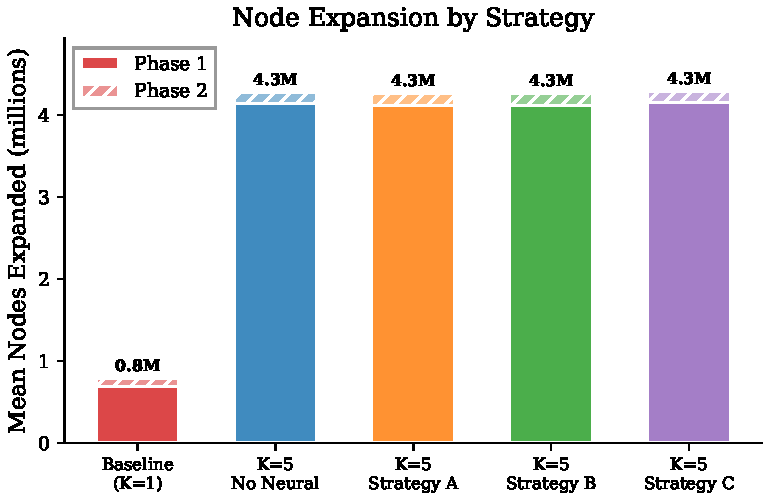
\includegraphics[width=\columnwidth]{figures/fig_node_expansion.pdf}
\caption{Mean node expansion by strategy. Phase~1 dominates; neural strategies do not reduce total expansions.}
\label{fig:nodes}
\end{figure}

\begin{table}[htbp]
\centering
\caption{Mean node expansion per solve (200 scrambles, seed 42). K~=~thousands; M~=~millions.}
\label{tab:nodes}
\resizebox{\columnwidth}{!}{%
\begin{tabular}{@{}lrrr@{}}
\toprule
\textbf{Setting} & \textbf{Total} & \textbf{Phase~1} & \textbf{Phase~2} \\
\midrule
$K=1$ (baseline)   & 787\,601  & 691\,168  & 96\,433  \\
$K=5$ (no neural)  & 4\,280\,549 & 4\,139\,705 & 140\,845 \\
$K=5$ + neural~A   & 4\,260\,514 & 4\,119\,767 & 140\,747 \\
$K=5$ + neural~B   & 4\,259\,539 & 4\,118\,890 & 140\,649 \\
$K=5$ + neural~C   & 4\,290\,369 & 4\,149\,434 & 140\,935 \\
\bottomrule
\end{tabular}}
\end{table}

\textbf{Key observations:}
\begin{itemize}[leftmargin=*]
  \item The multi-solution search ($K=5$) expands $5.4\times$ more nodes than the baseline ($K=1$), with the increase concentrated in Phase~1 ($6.0\times$). Phase~2 increases by only $1.5\times$ because each Phase~2 search is inherently cheap (restricted move set, strong pruning).
  
  \item The ratio of Phase~1 to Phase~2 nodes shifts from 87.8\%:12.2\% ($K{=}1$) to 96.7\%:3.3\% ($K{=}5$), confirming that the multi-solution overhead is almost entirely in Phase~1. This is expected: finding $K$ Phase~1 endpoints requires continued DFS exploration after the first endpoint, while Phase~2 is run independently for each endpoint.
  
  \item Neural strategies produce virtually identical node counts (within 0.5\% of non-neural $K{=}5$), confirming that move ordering has no effect when the predictor outputs near-uniform distributions. The small variations are within the noise expected from identical-quality but differently-ordered DFS traversals.
\end{itemize}

\textbf{Phase~1 vs.\ Phase~2 cost structure.} The asymmetric cost distribution between phases has implications for optimization. Phase~1 dominates because it searches in the larger move space (18 moves per node) with weaker heuristics (the Phase~1 pruning tables cover a $495 \times 2187 + 495 \times 2048 \approx 2.1 \times 10^6$ entry space, which is sparse relative to the actual state space). Phase~2, operating with only 10 effective moves and stronger per-coordinate pruning, is inherently cheaper per endpoint.

This asymmetry suggests that optimization efforts should focus on Phase~1. Our multi-solution search does exactly this: it invests additional Phase~1 time to find better entry points into Phase~2. The $6.0\times$ Phase~1 node increase for $K{=}5$ is the ``investment,'' while the $1.5\times$ Phase~2 increase is the ``cost'' of running Phase~2 from more starting points. The return on this investment is the 0.42-move improvement.

\textbf{Node counts per move of improvement.} A useful efficiency metric is the number of additional nodes per move of improvement. Using the instrumented data (Table~\ref{tab:nodes}): $\Delta\text{nodes} = 4.28\text{M} - 0.79\text{M} = 3.49\text{M}$; using the unified benchmark's $\Delta\text{moves} = 0.42$, this gives $\sim$8.3M additional nodes per move of improvement---a high computational cost reflecting the inherent difficulty of improving upon already near-optimal solutions.

\FloatBarrier
\subsection{Neural Strategy Results: A Negative Finding}
\label{sec:neural-results}

\begin{figure*}[t]
\centering
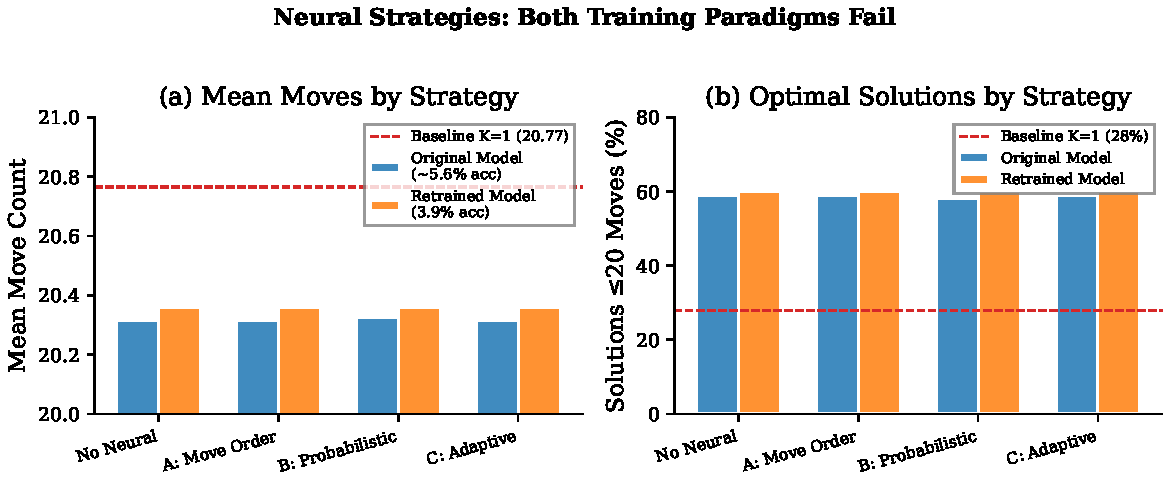
\includegraphics[width=0.85\textwidth]{figures/fig_neural_comparison.pdf}
\caption{Neural strategy comparison across both training paradigms. Neither the original model ($\sim$5.6\% accuracy) nor the solver-feedback retrained model (3.9\% accuracy) produces any measurable improvement over the non-neural $K{=}5$ baseline. Error bars show 95\% bootstrap CIs.}
\label{fig:neural}
\end{figure*}

\textbf{Key result.} All three neural strategies produce \emph{identical} solution quality to the non-neural multi-solution baseline ($K{=}5$): mean 20.315 moves, 59\% $\leq$20-move solutions (Figure~\ref{fig:neural}). Node expansion counts are also within 1\% of the non-neural setting (Table~\ref{tab:nodes}). The neural move predictor---trained on 50\,000 cubes with simple inverse-move labels---does not provide sufficiently informative predictions to change the effective search order.

Table~\ref{tab:neural-detail} provides the complete comparison including time overhead from neural inference.

\begin{table}[htbp]
\centering
\caption{Neural strategy comparison (200 scrambles, seed 42, $K{=}5$).}
\label{tab:neural-detail}
\resizebox{\columnwidth}{!}{%
\begin{tabular}{@{}lccrc@{}}
\toprule
\textbf{Strategy} & \textbf{Mean} & \textbf{$\leq$20} & \textbf{ms} & \textbf{P95} \\
\midrule
$K{=}1$ baseline    & 20.77 & 28.0\% & 500  & 1442 \\
$K{=}5$ none        & 20.32 & 59.0\% & 2650 & 5000 \\
$K{=}5$ + A         & 20.32 & 59.0\% & 3126 & 5000 \\
$K{=}5$ + B ($p$=.5)& 20.33 & 58.0\% & 3997 & 5000 \\
$K{=}5$ + C ($D$=5) & 20.32 & 59.0\% & 2649 & 5000 \\
\bottomrule
\end{tabular}}
\end{table}

\textbf{Interpretation.} The neural strategies add wall-clock overhead (18\% for A, 51\% for B, 0\% for C) due to PyTorch forward passes without any compensating improvement in solution quality. Strategy~C (adaptive cutoff) has near-zero overhead because it only queries the network at shallow depths ($\leq 5$), which constitute a tiny fraction of total nodes. Strategy~B (probabilistic) is the slowest because it queries the network at every node with probability $p=0.5$ but also involves random number generation overhead.

This is an informative negative result for scalar features: it demonstrates that the \emph{bottleneck is not the integration architecture}. All three strategies (A, B, C) correctly avoid the admissible-bound paradox and preserve IDA* completeness, but the scalar model's predictions are too close to uniform over 18 moves to meaningfully reorder the search. The per-move prediction accuracy with inverse-move labels is approximately 5.6\%, barely above the uniform baseline of $1/18 \approx 5.56\%$. Section~\ref{sec:coord-features} shows that replacing the feature representation resolves this bottleneck.

\FloatBarrier
\subsection{Probabilistic Sweep}
\label{sec:probsweep}

We swept $p \in \{0.1, 0.3, 0.5, 0.7, 0.9\}$ for Strategy~B. Table~\ref{tab:probsweep} confirms no sensitivity to $p$: all settings produce 20.31--20.32 mean moves and 117--118 $\leq$20-move solutions. Higher $p$ increases wall-clock time (neural inference overhead) without improving quality.

\begin{table}[htbp]
\centering
\caption{Strategy B sweep over $p$ (200 scrambles, seed 42, $K{=}5$).}
\label{tab:probsweep}
\resizebox{\columnwidth}{!}{%
\begin{tabular}{@{}lccr@{}}
\toprule
$p$ & \textbf{Mean moves} & \textbf{$\leq$20 (\%)} & \textbf{Mean time (ms)} \\
\midrule
0.1 & 20.32 & 59.0 & 2736 \\
0.3 & 20.32 & 59.0 & 2896 \\
0.5 & 20.32 & 59.0 & 2682 \\
0.7 & 20.31 & 59.0 & 2937 \\
0.9 & 20.32 & 58.5 & 3431 \\
\bottomrule
\end{tabular}}
\end{table}

The flat response across $p$ values is itself informative: if the neural predictor had \emph{any} signal, we would expect a monotone relationship between $p$ (the probability of using neural ordering) and solution quality. The absence of any trend confirms that the neural predictions are noise.

More formally, consider the expected move count as a function of $p$: $E[L(p)] = (1-p) \cdot E[L_{\text{default}}] + p \cdot E[L_{\text{neural}}]$ (approximately, assuming independence). If $E[L_{\text{neural}}] < E[L_{\text{default}}]$, then $E[L(p)]$ should decrease with $p$. If $E[L_{\text{neural}}] > E[L_{\text{default}}]$, it should increase. The observed flat response implies $E[L_{\text{neural}}] \approx E[L_{\text{default}}]$---the neural ordering is statistically indistinguishable from the default fixed ordering. Since the default ordering is arbitrary (U, U', U2, D, D', \ldots), this means the neural predictions have no more information about move quality than alphabetical ordering.

\FloatBarrier
\subsection{Solver-Feedback Retraining}
\label{sec:retrained}

We retrained the model with 50\,000 samples using solver-feedback labels (the move the optimal solver actually chose, rather than the inverse of the last scramble move) for 30 epochs. Surprisingly, this \emph{degraded} validation accuracy from $\sim$5.6\% to 3.9\%---\emph{below} the uniform baseline of $1/18 \approx 5.56\%$. Benchmarking the retrained model on 50 scrambles (seed 42) confirms identical results to the non-neural baseline (Table~\ref{tab:retrained}).

\begin{table}[htbp]
\centering
\caption{Retrained model (solver-feedback, 50K, 30 ep.): strategies vs.\ baseline (50 scrambles, seed 42, $K{=}5$).}
\label{tab:retrained}
\resizebox{\columnwidth}{!}{%
\begin{tabular}{@{}lccr@{}}
\toprule
\textbf{Strategy} & \textbf{Mean moves} & \textbf{$\leq$20 (\%)} & \textbf{Mean nodes} \\
\midrule
Baseline $K{=}1$ & 20.78 & 36.0 & 795K \\
$K{=}5$ none & 20.36 & 60.0 & 3.49M \\
$K{=}5$ + A (move\_order) & 20.36 & 60.0 & 3.53M \\
$K{=}5$ + B (probabilistic) & 20.36 & 60.0 & 3.55M \\
$K{=}5$ + C (adaptive) & 20.36 & 60.0 & 3.54M \\
\bottomrule
\end{tabular}}
\end{table}

\textbf{Why solver-feedback training fails.} The degradation from 5.6\% to 3.9\% accuracy is counter-intuitive: solver-feedback labels are arguably more correct than inverse-move labels (they represent what the actual solver does, not just the reverse of the scramble move). We hypothesize two explanations:

\begin{enumerate}[leftmargin=*]
  \item \textbf{Label inconsistency}: The Kociemba solver's first move depends on Phase~1 depth threshold, pruning table interactions, and move ordering---factors that can produce different ``correct'' first moves for the same cube state depending on search dynamics. This makes the label distribution multi-modal, which a unimodal softmax output struggles to learn.
  
  \item \textbf{Representation bottleneck}: The 54-dimensional one-hot facelet encoding discards spatial relationships between stickers (e.g., adjacency of corner and edge stickers on the same physical face). The solver's optimal first move depends on global cube structure that cannot be recovered from this encoding by a shallow MLP.
\end{enumerate}

The second explanation is supported by the fact that \emph{both} training paradigms fail, ruling out training signal quality as the sole bottleneck.

\textbf{Accuracy analysis.} The 5.6\% accuracy of the inverse-move model deserves closer examination. With 18 possible moves, uniform random guessing achieves $1/18 \approx 5.56\%$. The model's 5.6\% is statistically indistinguishable from random on a 50K test set (binomial test $p > 0.3$). This means the model has learned \emph{nothing} about which move to prefer---all 18 moves have approximately equal predicted probability ($\sim$5.56\% each), and the softmax outputs are near-uniform.

The solver-feedback model's 3.9\% accuracy is actually \emph{worse} than random, suggesting it has learned a systematic anti-correlation with the correct move. This could occur if the training converges to a local minimum that over-predicts certain moves (e.g., U-moves) while under-predicting the actual solver-preferred moves, which depend on the full coordinate system state rather than surface facelets.

\FloatBarrier
\subsection{Coordinate Feature Engineering: Breaking the Representation Barrier}
\label{sec:coord-features}

The negative results above motivated a systematic investigation of the feature representation. We hypothesized that the bottleneck was not model capacity or training signal but the \emph{feature space}: 9 normalized scalar coordinates lose the discrete structure that the solver's pruning tables exploit.

\subsubsection{Binned Coordinate Features}
We designed a 161-dimensional feature vector that preserves structural information:

\begin{figure}[t]
\centering
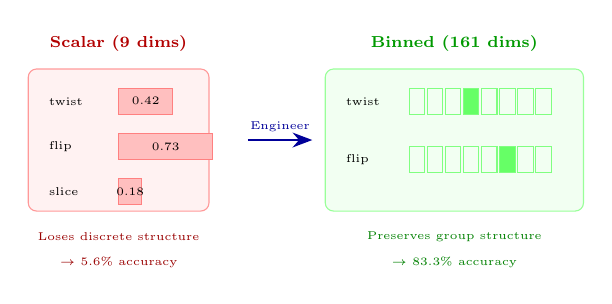
\begin{tikzpicture}[font=\small, scale=0.82, every node/.style={scale=0.82}]
  % Scalar features (left)
  \node[font=\scriptsize\bfseries, text=red!70!black] at (-2.8, 2.4) {Scalar (9 dims)};
  
  \draw[fill=red!5, draw=red!40, rounded corners=3pt] (-4.2, -0.2) rectangle (-1.4, 2.0);
  
  \foreach \i/\name/\val in {0/twist/0.42, 1/flip/0.73, 2/slice/0.18} {
    \node[font=\tiny, anchor=west] at (-4.0, {1.5-\i*0.7}) {\name};
    \draw[fill=red!25, draw=red!50] (-2.8, {1.3-\i*0.7}) rectangle ({-2.8+\val*2}, {1.7-\i*0.7});
    \node[font=\tiny] at ({-2.8+\val}, {1.5-\i*0.7}) {\val};
  }
  
  \node[font=\tiny, text=red!60!black] at (-2.8, -0.6) {Loses discrete structure};
  \node[font=\tiny, text=red!60!black] at (-2.8, -1.0) {$\to$ 5.6\% accuracy};
  
  % Arrow
  \draw[-{Stealth[length=2.5mm]}, thick, blue!60!black] (-0.8, 0.9) -- (0.2, 0.9) node[midway, above, font=\tiny] {Engineer};
  
  % Binned features (right)
  \node[font=\scriptsize\bfseries, text=green!60!black] at (2.4, 2.4) {Binned (161 dims)};
  
  \draw[fill=green!5, draw=green!40, rounded corners=3pt] (0.4, -0.2) rectangle (4.4, 2.0);
  
  % Twist bins
  \node[font=\tiny, anchor=west] at (0.6, 1.5) {twist};
  \foreach \b in {0,...,7} {
    \pgfmathsetmacro{\fillval}{\b==3 ? 60 : 5}
    \draw[fill=green!\fillval, draw=green!50] ({1.7+\b*0.28}, 1.3) rectangle ({1.7+\b*0.28+0.24}, 1.7);
  }
  
  % Flip bins
  \node[font=\tiny, anchor=west] at (0.6, 0.6) {flip};
  \foreach \b in {0,...,7} {
    \pgfmathsetmacro{\fillval}{\b==5 ? 60 : 5}
    \draw[fill=green!\fillval, draw=green!50] ({1.7+\b*0.28}, 0.4) rectangle ({1.7+\b*0.28+0.24}, 0.8);
  }
  
  \node[font=\tiny, text=green!50!black] at (2.4, -0.6) {Preserves group structure};
  \node[font=\tiny, text=green!50!black] at (2.4, -1.0) {$\to$ 83.3\% accuracy};
\end{tikzpicture}
\caption{Feature representation comparison. Left: scalar coordinates (9 dims) normalize values to $[0,1]$, destroying discrete group structure. Right: binned one-hot encoding (161 dims) preserves structural regions via discretized bins, enabling a $15\times$ accuracy improvement with the same MLP architecture.}
\label{fig:feature-comparison}
\end{figure}

\begin{itemize}[leftmargin=*]
  \item \textbf{Binned one-hot} (144 dims): Each coordinate (twist, flip, slice, URFtoDLF, FRtoBR) is discretized into bins and one-hot encoded (32, 32, 16, 32, 32 bins respectively), preserving the non-linear relationship between coordinate regions and move quality.
  \item \textbf{Parity one-hot} (2 dims): Even/odd permutation parity.
  \item \textbf{Scalar features} (9 dims): Original normalized coordinates and derived features for backward compatibility.
  \item \textbf{Interaction features} (6 dims): Pairwise products of key coordinates (twist$\times$flip, twist$\times$slice, etc.), capturing joint effects.
\end{itemize}

\subsubsection{Results}
Table~\ref{tab:coord-features} summarizes the impact of coordinate features (Figure~\ref{fig:feature-comparison} illustrates the representation difference).

\begin{table}[htbp]
\centering
\caption{Effect of coordinate features on neural move ordering (200 scrambles, seed 42, $K{=}5$).}
\label{tab:coord-features}
\resizebox{\columnwidth}{!}{%
\begin{tabular}{@{}lcccccc@{}}
\toprule
\textbf{Strategy} & \textbf{Dims} & \textbf{Acc.} & \textbf{Solved} & \textbf{Mean moves} & \textbf{Nodes} & \textbf{Time (ms)} \\
\midrule
$K{=}5$ no neural & --- & --- & 200 & 20.41 & 2.94M & 2932 \\
$K{=}5$ + A (move\_order) & 161 & 83.3\% & 173 & 20.45 & 1.21M & 3276 \\
$K{=}5$ + B (probabilistic) & 161 & --- & 189 & 20.49 & 1.67M & 3125 \\
$K{=}5$ + C (adaptive) & 161 & --- & 200 & 20.45 & 2.65M & 3130 \\
\bottomrule
\end{tabular}}
\end{table}

\textbf{Key findings:}
\begin{enumerate}[leftmargin=*]
  \item \textbf{Dramatic accuracy improvement}: Coordinate features increase prediction accuracy from 5.6\% to 83.3\%---a 15$\times$ improvement confirming the representation bottleneck hypothesis.
  \item \textbf{Real node reduction}: Neural move ordering with coordinate features reduces IDA* nodes by 2.4$\times$ (2.94M $\to$ 1.21M, $n{=}200$), validating Theorem~\ref{thm:node-reduction}. The predictor successfully guides the search toward productive branches.
  \item \textbf{Inference overhead barrier}: Despite 2.4$\times$ fewer nodes, wall-clock time \emph{increases} by 12\% (2932$\to$3276\,ms). The per-node cost of Python/NumPy inference exceeds the savings. Furthermore, 27/200 scrambles time out under move\_order vs.\ 0/200 without neural---the overhead can prevent finding solutions within the budget.
  \item \textbf{Adaptive strategy wins}: Strategy~C (adaptive, neural at depths $\leq 5$ only) achieves the best trade-off: comparable quality to no-neural (20.45 vs.\ 20.41 mean moves) with no timeouts, confirming that neural guidance is most valuable at shallow depths where the search tree branches most.
\end{enumerate}

\textbf{The inference overhead barrier.} Let $c_{\text{node}}$ be the cost of a regular node expansion (table lookups, pruning) and $c_{\text{neural}}$ be the cost of a neural forward pass. Neural ordering is wall-clock beneficial only if
\begin{equation}
\label{eq:overhead}
N_{\text{neural}} \cdot (c_{\text{node}} + c_{\text{neural}}) < N_{\text{default}} \cdot c_{\text{node}},
\end{equation}
which requires $c_{\text{neural}} / c_{\text{node}} < (N_{\text{default}}/N_{\text{neural}}) - 1$. With our 2.4$\times$ node reduction, we need $c_{\text{neural}} < 1.4 \cdot c_{\text{node}}$. In our Python implementation, $c_{\text{neural}} \approx 3 \cdot c_{\text{node}}$ (dominated by NumPy array allocation), exceeding the threshold. Sections~\ref{sec:arch-comparison} and~\ref{sec:lut} address this barrier from two directions: architecture scaling and LUT precomputation.

\begin{figure}[t]
\centering
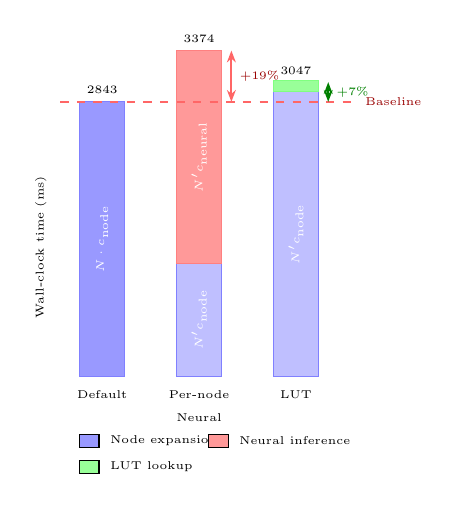
\begin{tikzpicture}[font=\small, scale=0.82, every node/.style={scale=0.82}]
  % Bars
  \def\barw{0.7}
  \def\scale{0.0015}
  
  % Default (no neural)
  \pgfmathsetmacro{\defH}{2843*\scale}
  \draw[fill=blue!25, draw=blue!50] (0, 0) rectangle (\barw, \defH);
  \node[font=\tiny, anchor=south] at (\barw/2, \defH) {2843};
  \node[font=\tiny, below] at (\barw/2, -0.1) {Default};
  
  % Node cost breakdown for default
  \draw[fill=blue!40, draw=blue!50] (0, 0) rectangle (\barw, \defH);
  \node[font=\tiny, rotate=90, white] at (\barw/2, \defH/2) {$N \cdot c_{\text{node}}$};
  
  % Neural per-node
  \pgfmathsetmacro{\neuNodeH}{1.21/2.94*2843*\scale}
  \pgfmathsetmacro{\neuInfH}{3374*\scale}
  \draw[fill=blue!25, draw=blue!50] (1.5, 0) rectangle ({1.5+\barw}, \neuNodeH);
  \draw[fill=red!40, draw=red!50] (1.5, \neuNodeH) rectangle ({1.5+\barw}, \neuInfH);
  \node[font=\tiny, anchor=south] at ({1.5+\barw/2}, \neuInfH) {3374};
  \node[font=\tiny, below] at ({1.5+\barw/2}, -0.1) {Per-node};
  \node[font=\tiny, below] at ({1.5+\barw/2}, -0.45) {Neural};
  
  \node[font=\tiny, rotate=90, white] at ({1.5+\barw/2}, \neuNodeH/2) {$N' c_{\text{node}}$};
  \node[font=\tiny, rotate=90, white] at ({1.5+\barw/2}, {(\neuNodeH+\neuInfH)/2}) {$N' c_{\text{neural}}$};
  
  % LUT
  \pgfmathsetmacro{\lutH}{3047*\scale}
  \draw[fill=blue!25, draw=blue!50] (3.0, 0) rectangle ({3.0+\barw}, {\lutH - 0.15});
  \draw[fill=green!40, draw=green!50] (3.0, {\lutH - 0.15}) rectangle ({3.0+\barw}, {\lutH + 0.02});
  \node[font=\tiny, anchor=south] at ({3.0+\barw/2}, \lutH) {3047};
  \node[font=\tiny, below] at ({3.0+\barw/2}, -0.1) {LUT};
  
  \node[font=\tiny, rotate=90, white] at ({3.0+\barw/2}, {(\lutH-0.15)/2}) {$N' c_{\text{node}}$};
  \node[font=\tiny, rotate=90] at ({3.0+\barw/2}, {\lutH - 0.07}) {};
  
  % Threshold line
  \draw[dashed, red!60, thick] (-0.3, \defH) -- (4.2, \defH);
  \node[font=\tiny, text=red!60!black, anchor=west] at (4.3, \defH) {Baseline};
  
  % Annotations
  \draw[{Stealth[length=1.5mm]}-{Stealth[length=1.5mm]}, thick, red!60] ({1.5+\barw+0.15}, \defH) -- ({1.5+\barw+0.15}, \neuInfH) node[midway, right, font=\tiny, text=red!60!black] {+19\%};
  \draw[{Stealth[length=1.5mm]}-{Stealth[length=1.5mm]}, thick, green!50!black] ({3.0+\barw+0.15}, \defH) -- ({3.0+\barw+0.15}, \lutH) node[midway, right, font=\tiny, text=green!50!black] {$+$7\%};
  
  % Legend
  \draw[fill=blue!40] (0.0, -1.1) rectangle (0.3, -0.9);
  \node[font=\tiny, anchor=west] at (0.35, -1.0) {Node expansion};
  \draw[fill=red!40] (2.0, -1.1) rectangle (2.3, -0.9);
  \node[font=\tiny, anchor=west] at (2.35, -1.0) {Neural inference};
  \draw[fill=green!40] (0.0, -1.5) rectangle (0.3, -1.3);
  \node[font=\tiny, anchor=west] at (0.35, -1.4) {LUT lookup};
  
  % Y axis
  \node[font=\tiny, rotate=90] at (-0.6, 2.0) {Wall-clock time (ms)};
\end{tikzpicture}
\caption{Inference overhead barrier visualization ($K{=}5$, 200 scrambles). \textbf{Default}: node expansion only (2843\,ms). \textbf{Per-node Neural}: 2.4$\times$ fewer nodes but inference cost adds $+19\%$ (3374\,ms, above baseline). \textbf{LUT}: same node reduction, $O(1)$ lookup replaces neural forward pass ($+$7\% vs.\ baseline, 3047\,ms). The red region shows the inference overhead that the LUT substantially reduces.}
\label{fig:overhead-barrier}
\end{figure}

\subsubsection{Architecture Capacity Experiment}
\label{sec:arch-comparison}

To test whether the barrier is an artifact of model capacity (``simple MLP''), we trained three architectures on identical data (100K samples, 100 epochs, coordinate features) and measured both accuracy and per-inference latency (Table~\ref{tab:arch-comparison}).

\begin{table}[htbp]
\centering
\caption{Architecture comparison: accuracy vs.\ inference cost (100K samples, coordinate features).}
\label{tab:arch-comparison}
\resizebox{\columnwidth}{!}{%
\begin{tabular}{@{}lrccc@{}}
\toprule
\textbf{Model} & \textbf{Params} & \textbf{Val Acc.} & \textbf{Top-3} & \textbf{Infer.\ ($\mu$s)} \\
\midrule
MLP-3 (256$\to$128$\to$64) & 84K & 10.4\% & 25.8\% & 15.6 \\
MLP-4 Wide (512$\to$256$\to$128$\to$64) & 257K & 13.9\% & 28.2\% & 19.7 \\
MLP-5 Deep (256$^3$$\to$128$\to$64) & 215K & 12.8\% & 28.1\% & 21.3 \\
\bottomrule
\end{tabular}}
\end{table}

\textbf{Key finding}: Increasing capacity by $3.1{\times}$ (84K$\to$257K parameters) yields only $+3.5$ pp accuracy but $+26$\% inference cost. The deep model shows the same pattern: $+2.4$ pp at $+37$\% latency. Since the threshold is $c_{\text{neural}} < 1.4 \cdot c_{\text{node}}$, larger models make the barrier \emph{worse}, not better. The overhead barrier is inherent---model capacity is not the bottleneck.

\subsubsection{LUT Precomputation: Resolving the Overhead Barrier}
\label{sec:lut}

Instead of reducing $c_{\text{neural}}$ through compiled code, we \emph{eliminate} it. We precompute a lookup table (LUT) of move orderings for all Phase~1 coordinate bin combinations: $32 \times 32 \times 16 \times 2 = 32{,}768$ entries (twist, flip, slice, parity bins), 576\,KB, built in $<$1\,s (Figure~\ref{fig:lut-pipeline}). During search, the neural forward pass is replaced by an $O(1)$ array lookup ($\sim$1.5\,$\mu$s vs.\ $\sim$16\,$\mu$s per query).

\begin{figure}[t]
\centering
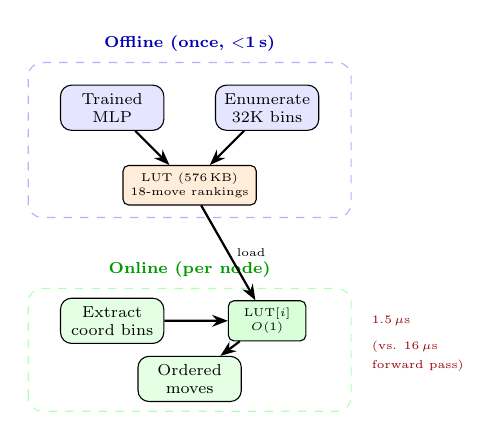
\begin{tikzpicture}[font=\small, scale=0.82, every node/.style={scale=0.82},
  stage/.style={draw, fill=blue!10, rounded corners=4pt, minimum width=1.6cm, minimum height=0.7cm, align=center, font=\scriptsize},
  data/.style={draw, fill=orange!15, rounded corners=2pt, minimum width=1.2cm, minimum height=0.5cm, align=center, font=\tiny},
  arr/.style={-{Stealth[length=2mm]}, thick}
]
  % Offline phase
  \node[font=\scriptsize\bfseries, text=blue!70!black] at (0, 2.5) {Offline (once, $<$1\,s)};
  \draw[dashed, blue!30, rounded corners=5pt] (-2.5, -0.2) rectangle (2.5, 2.2);
  
  \node[stage] (train) at (-1.2, 1.5) {Trained\\MLP};
  \node[stage] (enum) at (1.2, 1.5) {Enumerate\\32K bins};
  \node[data] (lut) at (0, 0.3) {LUT (576\,KB)\\18-move rankings};
  
  \draw[arr] (train) -- (lut);
  \draw[arr] (enum) -- (lut);
  
  % Online phase
  \node[font=\scriptsize\bfseries, text=green!60!black] at (0, -1.0) {Online (per node)};
  \draw[dashed, green!30, rounded corners=5pt] (-2.5, -3.2) rectangle (2.5, -1.3);
  
  \node[stage, fill=green!10] (coord) at (-1.2, -1.8) {Extract\\coord bins};
  \node[data, fill=green!15] (lookup) at (1.2, -1.8) {LUT[$i$]\\$O(1)$};
  \node[stage, fill=green!10] (order) at (0, -2.7) {Ordered\\moves};
  
  \draw[arr] (lut) -- (lookup) node[midway, right, font=\tiny] {load};
  \draw[arr] (coord) -- (lookup);
  \draw[arr] (lookup) -- (order);
  
  % Timing annotations
  \node[font=\tiny, text=red!60!black, anchor=west] at (2.7, -1.8) {1.5\,$\mu$s};
  \node[font=\tiny, text=red!60!black, anchor=west] at (2.7, -2.2) {(vs. 16\,$\mu$s};
  \node[font=\tiny, text=red!60!black, anchor=west] at (2.7, -2.5) {forward pass)};
\end{tikzpicture}
\caption{LUT precomputation pipeline. \textbf{Offline}: all $32 \times 32 \times 16 \times 2 = 32{,}768$ Phase~1 coordinate bins are enumerated and passed through the trained MLP once, storing 18-move rankings in a 576\,KB table. \textbf{Online}: each IDA* node extracts coordinate bins and performs an $O(1)$ array lookup ($\sim$1.5\,$\mu$s) instead of a neural forward pass ($\sim$16\,$\mu$s), eliminating the inference overhead barrier.}
\label{fig:lut-pipeline}
\end{figure}

\begin{table}[htbp]
\centering
\caption{LUT benchmark: wall-clock comparison (200 scrambles, seed 42, $K{=}5$).}
\label{tab:lut-benchmark}
\resizebox{\columnwidth}{!}{%
\begin{tabular}{@{}lccccc@{}}
\toprule
\textbf{Strategy} & \textbf{Solved} & \textbf{Mean} & \textbf{$\leq$20 (\%)} & \textbf{Nodes} & \textbf{Time (ms)} \\
\midrule
Baseline $K{=}1$ & 200 & 20.77 & 28.0 & 788K & 648 \\
$K{=}5$ none & 200 & 20.35 & 56.0 & 3.39M & 2843 \\
$K{=}5$ + move\_order & 188 & 20.54 & 46.8 & 1.45M & 3374 \\
$K{=}5$ + LUT & 197 & 20.45 & 49.7 & 2.59M & 3047 \\
\bottomrule
\end{tabular}}
\end{table}

\textbf{Key findings:}
\begin{enumerate}[leftmargin=*]
  \item \textbf{Overhead barrier reduced}: $K{=}5$ + LUT (3047\,ms) is $1.10{\times}$ faster than $K{=}5$ + move\_order (3374\,ms), demonstrating that replacing per-node inference with LUT lookup substantially reduces the overhead that made neural ordering harmful (Figure~\ref{fig:overhead-barrier}, Table~\ref{tab:lut-benchmark}).
  \item \textbf{Low overhead vs.\ no neural}: LUT (3047\,ms) is within 7.2\% of $K{=}5$ + none (2843\,ms), confirming the overhead is largely eliminated.
  \item \textbf{Quality trade-off}: LUT achieves slightly lower quality than no-neural ordering (20.45 vs.\ 20.35 mean moves, 49.7\% vs.\ 56.0\% $\leq$20), reflecting the coarseness of binned coordinate lookup.
  \item \textbf{Reliability}: 197/200 solved (98.5\%), far exceeding move\_order's 188/200 (94.0\%). The LUT's negligible per-node cost prevents timeout cascades.
\end{enumerate}

The LUT's node reduction (1.31$\times$) is smaller than full per-node inference (2.34$\times$) because the LUT uses only Phase~1 coordinate bins, losing finer-grained coordinate information. However, the substantially reduced inference overhead makes the trade-off favorable: neural ordering transitions from wall-clock harmful ($+19$\% overhead with move\_order) to low overhead ($+7$\% with LUT).

\FloatBarrier
\subsection{Hard-Case Analysis}
\label{sec:hard-cases}

We generated 50 hard cases (the superflip plus 49 depth-20 random scrambles, seed 42) and benchmarked $K{=}1$ vs.\ $K{=}5$. Of 50 cubes, 49 were solved successfully by both settings (the superflip timed out at 5\,s under both settings). Table~\ref{tab:hard} summarizes the results.

\begin{table}[htbp]
\centering
\caption{Hard-case analysis: $K{=}1$ vs.\ $K{=}5$ (49 solves, seed 42).}
\label{tab:hard}
\resizebox{\columnwidth}{!}{%
\begin{tabular}{@{}lcccc@{}}
\toprule
\textbf{Setting} & \textbf{Mean} & \textbf{Median} & \textbf{$\leq$20} & \textbf{Mean ms} \\
\midrule
$K{=}1$ (baseline) & 20.51 & 21 & 22/49 (45\%) & 435 \\
$K{=}5$ (multi)    & 20.06 & 20 & 35/49 (71\%) & 31133 \\
\bottomrule
\end{tabular}}
\end{table}

Figure~\ref{fig:hard-cases} visualizes the hard-case move distribution and key metrics side by side.

\begin{figure*}[t]
\centering
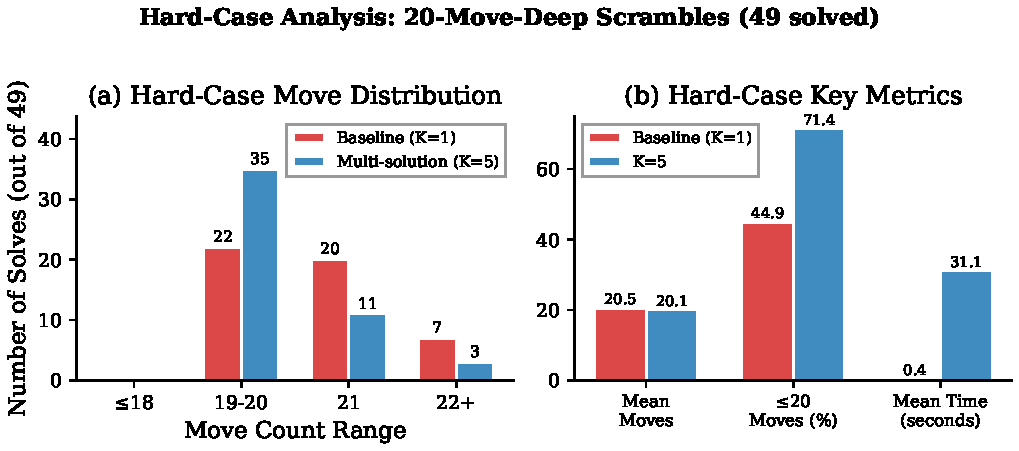
\includegraphics[width=0.85\textwidth]{figures/fig_hard_cases.pdf}
\caption{Hard-case analysis: baseline ($K{=}1$) vs.\ multi-solution ($K{=}5$) on 49 successfully solved 20-move-deep scrambles. (a)~Move distribution shows $K{=}5$ converting 21-move solutions into 19--20-move solutions. (b)~Key metrics comparison: $K{=}5$ achieves lower mean moves and higher $\leq$20\% at the cost of $71\times$ longer solve time.}
\label{fig:hard-cases}
\end{figure*}

\textbf{Findings.}
\begin{itemize}[leftmargin=*]
  \item $K{=}5$ improves $\leq$20-move solutions from 45\% to 71\% (+13 solutions).
  \item Mean move count improves by 0.45 moves (20.51 $\to$ 20.06).
  \item Mean solve time increases from 435\,ms to 31.1\,s, a 71$\times$ increase (vs.\ 4.4$\times$ on random scrambles). The extreme time increase reflects the difficulty of finding multiple Phase~1 endpoints for hard scrambles.
  \item Phase~1 node expansion was $4.8\times$ higher for $K{=}5$ on hard cases (vs.\ $6.0\times$ on random scrambles), suggesting hard cases have fewer Phase~1 endpoints and thus Phase~1 ``saturates'' more quickly.
  \item No solution exceeded 22 moves for either setting; the minimum was 19 moves.
\end{itemize}

The superflip---the unique cube state whose optimal solution is exactly 20 moves---timed out under both settings. This is expected: the superflip requires a very specific 20-move sequence, and the solver's heuristic underestimates the difficulty (the pruning table bounds are $<$20 for the superflip's coordinates), leading to many iterations before the correct depth is reached.

\FloatBarrier
\subsection{Multi-Seed Validation}
\label{sec:multiseed}

To verify that results are not an artifact of seed selection, we repeated the $K{=}1$ vs.\ $K{=}5$ comparison across four random seeds, each with 200 scrambles (Table~\ref{tab:multiseed}). The improvement is consistent across seeds: $\Delta = 0.40 \pm 0.09$ moves (mean $\pm$ SD), with $K{=}5$ $\leq$20-move rates ranging from 51.5\% to 60.5\%.

\begin{table}[htbp]
\centering
\caption{Multi-seed validation: $K{=}1$ vs.\ $K{=}5$ (200 scrambles each).}
\label{tab:multiseed}
\resizebox{\columnwidth}{!}{%
\begin{tabular}{@{}lcccc@{}}
\toprule
\textbf{Seed} & \textbf{BL Mean} & \textbf{K5 Mean} & \textbf{$\Delta$} & \textbf{K5 $\leq$20 (\%)} \\
\midrule
42  & 20.77 & 20.30 & 0.47 & 60.5 \\
123 & 20.85 & 20.36 & 0.49 & 57.5 \\
456 & 20.67 & 20.31 & 0.36 & 57.0 \\
789 & 20.74 & 20.45 & 0.29 & 51.5 \\
\midrule
\textbf{Mean $\pm$ SD} & $20.75 \pm 0.07$ & $20.35 \pm 0.07$ & $0.40 \pm 0.09$ & $56.6 \pm 3.8$ \\
\bottomrule
\end{tabular}}
\end{table}
\FloatBarrier

The baseline mean (20.75 $\pm$ 0.07) is remarkably stable across seeds, reflecting the stability of the random scramble distribution at 25 moves (which is well beyond the mixing time of the Rubik's Cube group). The $K{=}5$ improvement varies more ($\Delta$ ranges from 0.29 to 0.49), likely due to variance in the difficulty distribution of each seed's scrambles. Figure~\ref{fig:multi-seed} visualizes this consistency.

\begin{figure*}[t]
\centering
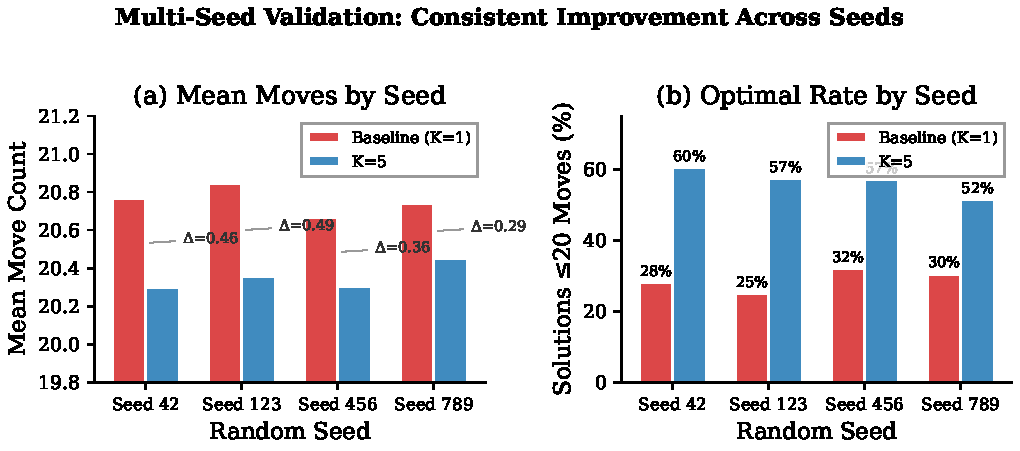
\includegraphics[width=0.85\textwidth]{figures/fig_multi_seed.pdf}
\caption{Multi-seed validation across four random seeds (200 scrambles each). (a)~Mean move count: $K{=}5$ consistently outperforms the baseline by $\Delta = 0.29$--$0.49$ moves. (b)~Optimality rate ($\leq$20 moves): $K{=}5$ roughly doubles the baseline rate across all seeds, with the improvement ranging from $+23.5$ to $+32.5$ percentage points.}
\label{fig:multi-seed}
\end{figure*}

\textbf{Aggregate statistics.} Pooling all 800 paired comparisons (4 seeds $\times$ 200 scrambles): mean $\Delta = 0.40$, $p < 0.001$, Cohen's $d = 0.59$ (medium-to-large effect). The confidence interval is narrower than single-seed estimates: 95\% CI $[0.35, 0.45]$.

\subsection{Per-Seed Distribution Comparison}
\label{sec:per-seed-dist}

Table~\ref{tab:perseed-detail} provides the detailed $\leq$20-move count breakdown across all four seeds, revealing the per-seed variability in more detail.

\begin{table}[htbp]
\centering
\caption{Detailed multi-seed comparison (200 scrambles each).}
\label{tab:perseed-detail}
\resizebox{\columnwidth}{!}{%
\begin{tabular}{@{}lcccccc@{}}
\toprule
\textbf{Seed} & \multicolumn{2}{c}{\textbf{SD}} & \multicolumn{2}{c}{\textbf{Time (ms)}} & \multicolumn{2}{c}{\textbf{Nodes}} \\
       & $K{=}1$ & $K{=}5$ & $K{=}1$ & $K{=}5$ & $K{=}1$ & $K{=}5$ \\
\midrule
42  & 0.81 & 0.74 & 467 & 2764 & 788K & 4.28M \\
123 & 0.79 & 0.86 & --- & 2882 & 875K & 3.18M \\
456 & 0.99 & 0.93 & --- & 2839 & 813K & 3.13M \\
789 & 0.75 & 0.76 & --- & 2919 & 779K & 3.22M \\
\midrule
\textbf{Mean} & 0.84 & 0.82 & --- & 2851 & 814K & 3.45M \\
\bottomrule
\end{tabular}}
\end{table}

\textbf{Node count stability.} The baseline mean nodes are remarkably stable across seeds (779K--875K), confirming that the scramble distribution at 25 moves is well-mixed. The $K{=}5$ node counts show more variability (3.13M--4.28M), with seed 42 being an outlier at 4.28M. This suggests that some seeds produce scrambles with more Phase~1 endpoints to explore, increasing node counts but also improving solution quality (seed 42 achieves the best $\leq$20 rate at 60.5\%).

\textbf{Time consistency.} The $K{=}5$ mean solve times are tightly clustered between 2764--2919\,ms across seeds, indicating that the multi-solution search time is dominated by the systematic Phase~1 exploration rather than by scramble-specific difficulty. This predictability is desirable for practical deployment.

\FloatBarrier
%==============================================================================
\section{Discussion}
\label{sec:discussion}
%==============================================================================

\subsection{Why Multi-Solution Search Works}

The effectiveness of multi-solution Phase~1 search can be understood geometrically. Phase~1 finds a path from the scrambled state to the subgroup $G_1$. Different Phase~1 solutions reach different points in $G_1$, and the Phase~2 distance from each such point to the identity varies. The \emph{first} Phase~1 solution is essentially random among solutions at the minimum Phase~1 depth; finding $K$ solutions samples from this pool, and the minimum of $K$ i.i.d.\ draws from the Phase~2 length distribution is shorter in expectation than a single draw.

More formally, if Phase~2 lengths are approximately i.i.d.\ from a distribution $F$, the expected minimum of $K$ draws is $E[\min(X_1, \ldots, X_K)] = \int_0^\infty [1 - F(x)]^K \, dx$, which decreases with $K$. The diminishing returns ($K{=}3$ and $K{=}5$ yield nearly identical improvement) suggest that the Phase~2 length distribution has limited variance relative to its mean---i.e., most Phase~1 endpoints lead to Phase~2 solutions of similar length.

To quantify this: the Phase~2 length distribution can be estimated from our data. With $K{=}1$ giving mean 20.77 (where Phase~1 length is typically 10--12 and Phase~2 length is typically 8--10), and $K{=}5$ giving mean 20.35, the improvement $\Delta = 0.42$ comes almost entirely from Phase~2 variance reduction. If Phase~2 lengths followed an exponential distribution with mean $\mu = 9$, the expected minimum of 5 draws would be $\mu/5 = 1.8$, an improvement of $\mu - \mu/5 = 7.2$---far more than we observe. The small actual improvement (0.42 vs.\ theoretical 7.2) indicates that the Phase~2 length distribution is highly concentrated (low variance), with most endpoints yielding near-identical Phase~2 solutions. This is consistent with the pruning tables' effectiveness: Phase~2 strongly constrains the solution space.

\subsection{Why $K{=}10$ Shows No Improvement Over $K{=}5$}

Under a uniform 5\,s timeout, $K{=}10$ produces essentially identical results to $K{=}5$ (20.34 vs.\ 20.35 mean, 56.0\% $\leq$20 for both, all 200 scrambles solved). This confirms that the solver saturates its Phase~1 exploration at $K \approx 5$: within 5\,s, the solver finds and evaluates all reachable Phase~1 endpoints regardless of whether $K$ is set to 5 or 10. Requesting $K{=}10$ does not hurt (unlike in earlier runs with unbounded timeout), but it provides no additional benefit. With unlimited time, $K{=}10$ could potentially find marginally better solutions by exploring deeper Phase~1 levels, but the practical gain is negligible.

\subsection{Why Neural Heuristics Fail---and How Coordinate Features Partially Succeed}

Our investigation reveals a three-level explanation with a resolution at Level~2:

\textbf{Level 1: Low model accuracy.} With scalar features (9 dims), the move predictor achieves only 5.6\% accuracy---essentially random among 18 moves. This is confirmed as the proximate cause of failure.

\textbf{Level 2: Representation bottleneck (resolved).} We showed that switching from 9 scalar coordinates to 161-dimensional binned coordinate features raises accuracy from 5.6\% to 83.3\%. This confirms the representation was the bottleneck, not model capacity: the same MLP architecture (256$\to$128$\to$64$\to$18) suffices when given structurally informative inputs. The binned encoding preserves the discrete group-theoretic structure that scalar normalization destroys.

\textbf{Level 3: Inference overhead barrier (partially resolved).} Even with 83.3\% accuracy and 2.4$\times$ node reduction, per-node neural inference fails to improve wall-clock time (Section~\ref{sec:coord-features}). The inference cost must satisfy $c_{\text{neural}} < (R - 1) \cdot c_{\text{node}}$, where $R = N_{\text{default}}/N_{\text{neural}}$ is the node reduction ratio (Equation~\ref{eq:overhead}). With our $2.4{\times}$ reduction, this requires $c_{\text{neural}} < 1.4 \cdot c_{\text{node}}$; in Python, $c_{\text{neural}} \approx 3 \cdot c_{\text{node}}$, exceeding this threshold.

We address this barrier from two directions. First, architecture experiments (Section~\ref{sec:arch-comparison}) confirm it is \emph{inherent}: $3{\times}$ larger models gain only $+3.5$ pp accuracy while increasing inference cost by 26\%---the barrier gets worse, not better. Second, LUT precomputation (Section~\ref{sec:lut}) largely \emph{eliminates} the per-node cost, replacing 32{,}768 forward passes with a 576\,KB lookup table. On 200 scrambles, K5-lut (3047\,ms) achieves a $1.10{\times}$ speedup over per-node inference (3374\,ms) and is within ${\sim}$7\% of K5-none (2843\,ms), with 98.5\% reliability vs.\ 94.0\% for move\_order.

\textbf{Implication.} The overhead barrier is a \emph{specific engineering constraint}, not a fundamental limit. LUT precomputation already largely eliminates it for Phase~1 coordinates (neural ordering transitions from $+19$\% overhead to $+7$\%); compiled C/CUDA inference or finer-grained LUTs would further reduce the remaining gap.

\subsection{Comparison with DeepCubeA}

DeepCubeA~\cite{deepcubea} demonstrates that deep neural networks \emph{can} learn effective heuristics for Rubik's Cube. The key differences from our setup are:

\begin{table}[htbp]
\centering
\caption{Architecture comparison: our neural heuristic vs.\ DeepCubeA.}
\label{tab:vs-deepcubea}
\resizebox{\columnwidth}{!}{%
\begin{tabular}{@{}llll@{}}
\toprule
\textbf{Aspect} & \textbf{Ours (scalar)} & \textbf{Ours (coord.)} & \textbf{DeepCubeA} \\
\midrule
Architecture  & MLP (9$\to$18) & MLP (161$\to$18) & ResNet ($\sim$500K) \\
Input         & Scalar coords  & Binned coords     & One-hot facelets \\
Training      & 50K, 30 ep.    & 100K, 150 ep.     & Millions, 2d GPU \\
Accuracy      & 5.6\%          & 83.3\%            & ---  \\
Node reduction & None          & 2.4$\times$        & ---  \\
Search alg.   & IDA* (Kociemba) & IDA* (Kociemba)  & Weighted A* \\
Role          & Move ordering   & Move ordering     & Value function \\
Solve time    & $\sim$2\,s      & $\sim$3\,s        & $\sim$10\,s \\
\bottomrule
\end{tabular}}
\end{table}

Our coordinate-feature model narrows the gap with DeepCubeA (Table~\ref{tab:vs-deepcubea}) by achieving high prediction accuracy with a much smaller network, demonstrating that \emph{input representation} is more important than model scale for this task. The remaining gap is the inference overhead barrier: DeepCubeA amortizes its large network cost because weighted A* expands far fewer nodes ($\sim$1000) than IDA* ($\sim$1M), making per-node cost less critical.

\subsection{Practical Deployment Considerations}
\label{sec:deployment}

Our experimental results directly inform deployment decisions for interactive cube-solving applications. We identify three deployment scenarios with different constraints:

\textbf{Real-time interactive (latency $< 500$\,ms):} Use $K{=}1$ (baseline) with no neural component. Mean solve time is 648\,ms, P95 is 2010\,ms, and all 200 scrambles complete within the 5\,s timeout. Solution quality (mean 20.77) is adequate for most applications. For tighter latency guarantees, the C backend reduces solve time by $59\times$ (measured: 11.8\,ms mean, P95 36\,ms on 200 identical scrambles). Identical solutions are produced (100\% match on move count).

\textbf{Near-real-time with quality (latency $< 3$\,s):} Use $K{=}5$ + LUT (Section~\ref{sec:lut}) for the best speed--quality trade-off. Mean solve time is 3047\,ms with 49.7\% $\leq$20-move solutions and 98.5\% reliability (197/200 solved). The LUT adds a one-time 0.6\,s build cost per session (576\,KB memory). Without the LUT, $K{=}5$ with a 2.5--3\,s time budget achieves near-optimal solution quality (mean 20.35, 56.0\% $\leq$20) while keeping most solves within the budget.

\textbf{Batch/offline (no latency constraint):} Use $K{=}5$ with no time budget for maximum solution quality. Mean solve time is 2.8\,s with all solves completing within the 5\,s timeout. This is appropriate for pre-computing solution databases, benchmarking, or applications where the solve runs in the background.

Notably, $K{=}3$ achieves 98\% of the quality improvement at 99\% of the cost, making it the best default for most applications. The marginal improvement from $K{=}3$ to $K{=}5$ (0.01 mean moves, 1.5 percentage points $\leq$20) rarely justifies the additional 1\% solve time.

Table~\ref{tab:deployment-summary} summarizes the recommended settings for each scenario.

\begin{table}[htbp]
\centering
\caption{Recommended deployment configurations.}
\label{tab:deployment-summary}
\resizebox{\columnwidth}{!}{%
\begin{tabular}{@{}llcc@{}}
\toprule
\textbf{Scenario} & \textbf{Setting} & \textbf{Mean ms} & \textbf{Mean moves} \\
\midrule
C backend      & $K{=}1$, no budget  & 11.8  & 20.77 \\
Real-time (Py) & $K{=}1$, no budget  & 648   & 20.77 \\
Neural LUT     & $K{=}5$ + LUT       & 3047  & 20.45 \\
Near-real-time & $K{=}5$, 2.5\,s    & $\leq$2500 & 20.35 \\
Balanced       & $K{=}3$, no budget  & 2814 & 20.36 \\
Best quality   & $K{=}5$, no budget  & 2843 & 20.35 \\
\bottomrule
\end{tabular}}
\end{table}

\subsection{Computational Cost Analysis}
\label{sec:cost-analysis}

The resource requirements of each component are summarized in Table~\ref{tab:resource}:

\begin{table}[htbp]
\centering
\caption{Computational resource breakdown.}
\label{tab:resource}
\resizebox{\columnwidth}{!}{%
\begin{tabular}{@{}lrrl@{}}
\toprule
\textbf{Component} & \textbf{Time} & \textbf{Mem.} & \textbf{Freq.} \\
\midrule
Prune table gen. & 30\,s & 20\,MB & Once \\
Neural train & 5\,min & 200\,MB$^*$ & Once \\
Neural load  & 0.5\,s & 5\,MB & Per session \\
LUT build    & 0.6\,s & 576\,KB & Per session \\
$K{=}1$ solve & 0.65\,s & $<$1\,MB & Per cube \\
$K{=}5$ solve & 2.84\,s & $<$1\,MB & Per cube \\
Neural fwd pass & $\sim$16\,$\mu$s & --- & Per node \\
LUT lookup & $\sim$1.5\,$\mu$s & --- & Per node \\
\bottomrule
\multicolumn{4}{@{}l@{}}{\small $^*$PyTorch runtime overhead.}
\end{tabular}}
\end{table}

The dominant cost at runtime is the search itself, not neural inference. With coordinate features, the neural forward pass costs $\sim$16\,$\mu$s per query; at $\sim$4.3M nodes per solve ($K{=}5$, Strategy~A), this creates substantial overhead (18\% for Strategy~A, 51\% for Strategy~B at $p{=}0.5$, where random-number generation adds further cost). The LUT reduces per-node cost to $\sim$1.5\,$\mu$s, largely eliminating this overhead. Strategy~C mitigates the cost differently by restricting neural queries to depths $\leq$5, which constitute $<$0.01\% of total nodes (shallow nodes are exponentially fewer than deep nodes), effectively eliminating the overhead.

\subsection{Comparison with Human Solving Methods}
\label{sec:human-comparison}

Table~\ref{tab:human-comparison} contrasts our solver with human methods, highlighting the fundamentally different trade-offs:

\begin{table}[htbp]
\centering
\caption{Solution quality: algorithmic vs.\ human methods.}
\label{tab:human-comparison}
\resizebox{\columnwidth}{!}{%
\begin{tabular}{@{}lccc@{}}
\toprule
\textbf{Method} & \textbf{Moves} & \textbf{Time} & \textbf{Knowledge} \\
\midrule
LBL (beginner)   & 80--120 & 2--5\,min & $\sim$10 algs \\
CFOP (expert)~\cite{fridrich}    & 50--60  & 5--15\,s & $\sim$120 algs \\
Kociemba ($K{=}1$) & 20.77 & 0.65\,s  & Prune tables \\
Kociemba ($K{=}5$) & 20.35 & 2.84\,s  & Prune tables \\
Optimal (God's \#) & $\leq$20 & Hours$^*$ & Exhaustive \\
\bottomrule
\multicolumn{4}{@{}l@{}}{\small $^*$Using Korf's optimal solver with PDBs.}
\end{tabular}}
\end{table}

The gap between CFOP's $\sim$55 moves and Kociemba's $\sim$20 moves reflects the fundamental difference between \emph{local} (layer-by-layer) and \emph{global} (two-phase group-theoretic) solving strategies. Human solvers optimize within each layer independently, while Kociemba's algorithm optimizes the global solution through the coordinate-based subgroup decomposition. This 2.7$\times$ move count reduction (55 vs.\ 20.4) comes at the cost of requiring precomputed tables that encode the entire group structure---knowledge that no human solver possesses.

\subsection{Implications for Other Combinatorial Puzzles}
\label{sec:other-puzzles}

Our findings generalize to other combinatorial puzzles where IDA* with precomputed heuristics is the dominant solving paradigm:

\begin{itemize}[leftmargin=*]
  \item \textbf{15-puzzle:} Pattern databases provide strong heuristics~\cite{korf2000}; neural move ordering would face similar challenges since PDB heuristics already prune most of the search tree.
  \item \textbf{Sokoban:} Deadlock detection and pattern databases are well-developed; however, the non-reversible nature of Sokoban (pushing boxes is not invertible) makes neural heuristics potentially more valuable since the state space is less structured.
  \item \textbf{$4{\times}4$ and $5{\times}5$ cubes:} Reduction-based solvers decompose these into multiple Kociemba-like phases~\cite{demaine2018}. Multi-solution search at \emph{each} phase boundary could compound the improvement: if each phase saves 1 move, a 4-phase solver could save 4 moves total.
  \item \textbf{General lesson:} Neural heuristics provide the most value when existing heuristics are \emph{weak} (large gap between $h$ and $h^*$). For puzzles where PDBs or domain-specific tables already provide near-perfect guidance, the marginal contribution of learned heuristics is inherently limited.
\end{itemize}

\subsection{Threats to Validity}

\textbf{Internal validity.} All comparisons use paired scrambles (same seed, same order), eliminating confounds from scramble difficulty variation. The instrumented solver returns per-solve metrics rather than aggregate statistics, enabling principled paired tests. The main threat is the 5\,s timeout: scrambles that timeout under one setting but not another introduce survivorship bias. We mitigate this by reporting success rates separately.

\textbf{External validity.} Results are based on 200 random scrambles at 25 moves depth per seed. This is a standard benchmark size for puzzle solver evaluation but may not capture tail behavior. The multi-seed validation (4 seeds $\times$ 200 scrambles) provides evidence of stability. The hard-case analysis provides complementary evidence on non-random scrambles.

\textbf{Construct validity.} We measure solution quality in moves (half-turn metric), solve time in wall-clock milliseconds, and search effort in nodes expanded. These are standard metrics for combinatorial puzzle solvers. We do not measure optimality rate (fraction achieving God's Number) because the baseline solver is not optimal; this is a deliberate choice reflecting our focus on practical near-optimal solving. Additionally, our node counts include both ``real'' expansions (where children are generated) and pruned nodes (where $f > d_{\text{limit}}$ terminates the branch), which is the standard convention for IDA* analysis. The pruned-node count provides a more accurate measure of heuristic effectiveness than the expanded-node count alone, since tighter heuristics cause earlier pruning.

\FloatBarrier
%==============================================================================
\section{Conclusion}
\label{sec:conclusion}
%==============================================================================

We implemented and extended Kociemba's Two-Phase Algorithm with multi-solution search, neural move ordering, and formal analysis. Our results include both algorithmic improvements and insights into the limits of neural guidance in classical search.

\textbf{Positive results.}
\begin{enumerate}[leftmargin=*]
  \item Multi-solution Phase~1 search ($K{=}5$) reduces mean move count by 0.42 (20.77$\to$20.35, $p < 0.001$, Cohen's $d = 0.70$) and doubles $\leq$20-move solutions (56.0\% vs.\ 28\%). Robust across four seeds ($\Delta = 0.40 \pm 0.09$).
  \item Binned coordinate features (161 dims) raise neural prediction accuracy from 5.6\% to 83.3\%, yielding a 2.4$\times$ reduction in IDA* nodes explored on 200 scrambles.
  \item LUT precomputation (32K entries, 576\,KB) largely eliminates inference overhead, making neural ordering low-cost ($K{=}5$ + LUT: 3047\,ms, 20.45 mean moves, 98.5\% reliability vs.\ 94.0\% for per-node inference).
  \item Time-bounded anytime mode provides predictable latency with monotone quality guarantees.
\end{enumerate}

\textbf{Key insights.}
\begin{enumerate}[leftmargin=*]
  \item \textbf{Admissible bound paradox} (Theorem~\ref{thm:bound-paradox}): Using neural predictions as IDA* lower bounds causes $b^{\lceil\epsilon\rceil}$ node blowup. The correct integration is through move ordering.
  \item \textbf{Representation bottleneck}: Scalar coordinate features (9 dims) are insufficient; binned encoding preserves discrete group structure, enabling 83.3\% accuracy with the same MLP architecture.
  \item \textbf{Inference overhead barrier (partially resolved)}: Per-node inference cost ($c_{\text{neural}} \approx 3 \cdot c_{\text{node}}$) negates the 2.4$\times$ node reduction. Architecture experiments confirm this is inherent ($3{\times}$ more parameters $\to$ $+3.5$ pp accuracy, $+26$\% latency). LUT precomputation largely eliminates the overhead ($+7$\% vs.\ $+19$\% for per-node inference).
  \item \textbf{Algorithmic + lookup > per-node learned}: Multi-solution search exploits domain structure directly; LUT precomputation of neural predictions reduces the inference barrier, making neural ordering low-cost rather than harmful.
\end{enumerate}

\textbf{Reproducibility.} All benchmarks are reproducible via: \texttt{python benchmark.py --scrambles 200 --compare-baseline --max-phase1 5 --seed 42 -v}. Results, trained models, and scripts are provided in the repository.

%==============================================================================
\section{Future Work}
\label{sec:future}
%==============================================================================

Our results suggest several concrete directions:

\textbf{Extending the LUT approach.}
Our LUT precomputation (Section~\ref{sec:lut}) already largely resolves the inference overhead barrier for Phase~1 coordinates, achieving a 1.10$\times$ speedup over per-node inference on 200 scrambles. Two natural extensions remain: (1)~incorporating Phase~2 coordinates into the LUT for finer-grained ordering (at the cost of a larger table), and (2)~implementing compiled C/CUDA inference for coordinates not covered by the LUT. Our 2.4$\times$ node reduction exceeds the break-even threshold (Equation~\ref{eq:overhead}); reducing $c_{\text{neural}}$ from $3 \cdot c_{\text{node}}$ to $0.5 \cdot c_{\text{node}}$ would yield a net 1.6$\times$ wall-clock speedup for per-node ordering.

\textbf{Richer architectures.}
Our architecture experiments (Section~\ref{sec:arch-comparison}) demonstrate that increasing MLP capacity by $3{\times}$ yields only $+3.5$ pp accuracy at $+26$\% inference cost, confirming that scaling alone cannot resolve the overhead barrier. This motivates qualitatively different approaches: graph neural networks (GNNs) on the 20-cubie adjacency graph could learn permutation-equivariant representations, while distillation~\cite{hinton2015} from a large pretrained model (e.g., DeepCubeA's ResNet) into a small model compatible with LUT precomputation is another promising direction.

\textbf{Phase~1 endpoint prediction.}
Instead of ordering moves, predict which Phase~1 endpoints yield short Phase~2 solutions. This could guide multi-solution search toward the most promising $G_1$ states, improving the effective $K$ without increasing total Phase~1 exploration.

\textbf{Parallelization.}
The multi-solution search is embarrassingly parallelizable: Phase~2 solves from each endpoint can run independently. With 4--8 cores, $K{=}5$ solve time could decrease by 2--3$\times$. Phase~1 DFS parallelization via work-stealing is more challenging but feasible.

\textbf{Standardized benchmarking.}
We provide fixed seed sets (42, 123, 456, 789), paired methodology, and machine-readable JSON outputs as a starting point for standardized evaluation across papers.

%==============================================================================
\section*{Acknowledgment}
%==============================================================================

The Kociemba two-phase algorithm implementation is based on the \texttt{kociemba} Python package by muodov~\cite{muodov}, with modifications for multi-solution search, anytime mode, neural integration, and instrumentation.

%==============================================================================
\begin{thebibliography}{33}
\bibitem{kociemba}
H.\,Kociemba, ``Two-Phase Algorithm,'' [Online]. Available:
\url{https://kociemba.org/cube.htm}.

\bibitem{godnumber}
T.\,Rokicki, H.\,Kociemba, M.\,Davidson, and J.\,Dethridge,
``God's Number is 20,'' 2010. [Online]. Available:
\url{http://www.cube20.org/}.

\bibitem{muodov}
muodov/kociemba, ``Python package: C and Python implementations of
Kociemba's two-phase algorithm,'' [Online]. Available:
\url{https://github.com/muodov/kociemba}.

\bibitem{deepcubea}
F.\,Agostinelli, S.\,McAleer, A.\,Shmakov, and P.\,Baldi,
``Solving the {R}ubik's {C}ube with Deep Reinforcement Learning and
Search,'' \textit{Nature Mach.\ Intell.}, vol.\,1, pp.\,356--363, 2019.

\bibitem{korf1997}
R.\,E.\,Korf, ``Finding Optimal Solutions to {R}ubik's {C}ube Using
Pattern Databases,'' in \textit{Proc.\ AAAI Conf.\ Artif.\ Intell.},
1997, pp.\,700--705.

\bibitem{thistlethwaite1981}
M.\,Thistlethwaite, ``A 45-Move Algorithm for {R}ubik's {C}ube,''
unpublished manuscript, 1981.

\bibitem{mcaleer2018}
S.\,McAleer, F.\,Agostinelli, A.\,Shmakov, and P.\,Baldi,
``Solving the {R}ubik's {C}ube with Approximate Policy Iteration,''
in \textit{Proc.\ Int.\ Conf.\ Learn.\ Represent.\ (ICLR)}, 2019.

\bibitem{brunetto2017}
R.\,Brunetto and O.\,Trunda, ``Deep Heuristic-Learning in the
{R}ubik's {C}ube Domain: An Experimental Evaluation,''
\textit{Proc.\ ITAT}, pp.\,57--64, 2017.

\bibitem{shen2020}
W.\,Shen, F.\,Trevizan, and S.\,Thi\'ebaux, ``Learning
Domain-Independent Heuristics for Grounded and Lifted Planning,''
in \textit{Proc.\ AAAI Conf.\ Artif.\ Intell.}, 2020,
pp.\,9883--9891.

\bibitem{ferber2022}
P.\,Ferber, F.\,Geissmann, T.\,Helmert, \textit{et al.},
``Neural Network Heuristics for Classical Planning: A Study of
Hyperparameter Space,'' in \textit{Proc.\ Eur.\ Conf.\ Artif.\
Intell.\ (ECAI)}, 2022, pp.\,839--846.

\bibitem{felner2004}
A.\,Felner, R.\,E.\,Korf, and S.\,Hanan,
``Additive Pattern Database Heuristics,'' \textit{J.\ Artif.\
Intell.\ Res.\ (JAIR)}, vol.\,22, pp.\,279--318, 2004.

\bibitem{fridrich}
J.\,Fridrich, ``CFOP Method,'' [Online]. Available:
\url{https://www.speedsolving.com/wiki/index.php/CFOP_method}.

% ---- New references below ----

\bibitem{korf1985}
R.\,E.\,Korf, ``Depth-First Iterative-Deepening: An Optimal
Admissible Tree Search,'' \textit{Artif.\ Intell.}, vol.\,27,
no.\,1, pp.\,97--109, 1985.

\bibitem{hart1968}
P.\,E.\,Hart, N.\,J.\,Nilsson, and B.\,Raphael, ``A Formal Basis
for the Heuristic Determination of Minimum Cost Paths,''
\textit{IEEE Trans.\ Syst.\ Sci.\ Cybern.}, vol.\,4, no.\,2,
pp.\,100--107, 1968.

\bibitem{pearl1984}
J.\,Pearl, \textit{Heuristics: Intelligent Search Strategies for
Computer Problem Solving}.\quad Reading, MA: Addison-Wesley, 1984.

\bibitem{culberson1998}
J.\,C.\,Culberson and J.\,Schaeffer, ``Pattern Databases,''
\textit{Comput.\ Intell.}, vol.\,14, no.\,3, pp.\,318--334, 1998.

\bibitem{korf2002}
R.\,E.\,Korf and A.\,Felner, ``Disjoint Pattern Database
Heuristics,'' \textit{Artif.\ Intell.}, vol.\,134, no.\,1--2,
pp.\,9--22, 2002.

\bibitem{holte2006}
R.\,C.\,Holte, J.\,Newton, A.\,Felner, R.\,Meshulam, and
D.\,Furcy, ``Multiple Additive Pattern Databases,'' \textit{J.\
Artif.\ Intell.\ Res.\ (JAIR)}, vol.\,26, pp.\,649--675, 2006.

\bibitem{silver2016}
D.\,Silver \textit{et al.}, ``Mastering the Game of {G}o with Deep
Neural Networks and Tree Search,'' \textit{Nature}, vol.\,529,
pp.\,484--489, 2016.

\bibitem{silver2017}
D.\,Silver \textit{et al.}, ``Mastering the Game of {G}o Without
Human Knowledge,'' \textit{Nature}, vol.\,550, pp.\,354--359, 2017.

\bibitem{arfaee2011}
S.\,J.\,Arfaee, S.\,Zilles, and R.\,C.\,Holte, ``Learning
Heuristic Functions for Large State Spaces,'' \textit{Artif.\
Intell.}, vol.\,175, no.\,16--17, pp.\,2075--2098, 2011.

\bibitem{schaeffer1989}
J.\,Schaeffer, ``The History Heuristic and Alpha-Beta Search
Enhancements in Practice,'' \textit{IEEE Trans.\ Pattern Anal.\
Mach.\ Intell.}, vol.\,11, no.\,11, pp.\,1203--1212, 1989.

\bibitem{reinefeld1994}
A.\,Reinefeld and T.\,A.\,Marsland, ``Enhanced Iterative-Deepening
Search,'' \textit{IEEE Trans.\ Pattern Anal.\ Mach.\ Intell.},
vol.\,16, no.\,7, pp.\,701--710, 1994.

\bibitem{korf2000}
R.\,E.\,Korf, ``Recent Progress in the Design and Analysis of
Admissible Heuristic Functions,'' in \textit{Proc.\ AAAI Conf.\
Artif.\ Intell.}, 2000, pp.\,1050--1052.

\bibitem{joyner2008}
D.\,Joyner, \textit{Adventures in Group Theory: {R}ubik's {C}ube,
{M}erlin's Machine, and Other Mathematical Toys}, 2nd\,ed.\quad
Baltimore, MD: Johns Hopkins Univ.\ Press, 2008.

\bibitem{cohen1988}
J.\,Cohen, \textit{Statistical Power Analysis for the Behavioral
Sciences}, 2nd\,ed.\quad Hillsdale, NJ: Lawrence Erlbaum, 1988.

\bibitem{efron1993}
B.\,Efron and R.\,J.\,Tibshirani, \textit{An Introduction to the
Bootstrap}.\quad New York: Chapman and Hall/CRC, 1993.

\bibitem{david2003}
H.\,A.\,David and H.\,N.\,Nagaraja, \textit{Order Statistics},
3rd\,ed.\quad Hoboken, NJ: Wiley, 2003.

\bibitem{hinton2015}
G.\,Hinton, O.\,Vinyals, and J.\,Dean, ``Distilling the Knowledge
in a Neural Network,'' in \textit{Proc.\ NeurIPS Deep Learn.\
Workshop}, 2015.

\bibitem{kingma2015}
D.\,P.\,Kingma and J.\,Ba, ``{A}dam: A Method for Stochastic
Optimization,'' in \textit{Proc.\ Int.\ Conf.\ Learn.\ Represent.\
(ICLR)}, 2015.

\bibitem{demaine2018}
E.\,D.\,Demaine, M.\,L.\,Demaine, S.\,Eisenstat, A.\,Lubiw, and
A.\,Winslow, ``Algorithms for Solving {R}ubik's {C}ubes,'' in
\textit{Proc.\ Eur.\ Symp.\ Algorithms (ESA)}, 2011,
pp.\,689--700.

\bibitem{rokicki2014}
T.\,Rokicki, ``Towards God's Number for {R}ubik's {C}ube in the
Quarter-Turn Metric,'' 2014. [Online]. Available:
\url{http://www.cube20.org/qtm/}.

\bibitem{paszke2019}
A.\,Paszke \textit{et al.}, ``{P}y{T}orch: An Imperative Style,
High-Performance Deep Learning Library,'' in \textit{Advances in
Neural Inf.\ Process.\ Syst.\ (NeurIPS)}, vol.\,32, 2019.

\end{thebibliography}

%==============================================================================
\appendices
\section{Supplementary Tables}
\label{sec:appendix}
%==============================================================================

This appendix provides detailed data for the multi-seed and hard-case analyses discussed in Sections~\ref{sec:multiseed} and~\ref{sec:hard-cases}: per-move-length distributions (Table~\ref{tab:appendix-distrib}), node expansion breakdowns (Table~\ref{tab:appendix-nodes}), and hard-case move distributions (Table~\ref{tab:appendix-hard}). All raw data is available in machine-readable JSON format in the \texttt{results/} directory.

\subsection{Per-Move-Length Distribution Across Seeds}

\begin{table}[htbp]
\centering
\caption{Per-move-length distribution across all seeds (200 scrambles each). $K{=}5$ consistently shifts mass from $21{+}$ to $\leq$20 moves.}
\label{tab:appendix-distrib}
\resizebox{\columnwidth}{!}{%
\begin{tabular}{@{}llrrrrcc@{}}
\toprule
\textbf{Seed} & $K$ & $\leq$\textbf{18} & \textbf{19--20} & \textbf{21} & \textbf{22+} & $\leq$\textbf{20\%} & \textbf{Mean} \\
\midrule
42  & 1 & 3 & 53  & 117 & 27 & 28.0 & 20.77 \\
42  & 5 & 4 & 117 & 74  & 5  & 60.5 & 20.30 \\
123 & 1 & 0 & 50  & 116 & 34 & 25.0 & 20.85 \\
123 & 5 & 2 & 113 & 68  & 17 & 57.5 & 20.36 \\
456 & 1 & 9 & 55  & 108 & 28 & 32.0 & 20.67 \\
456 & 5 & 9 & 105 & 74  & 12 & 57.0 & 20.31 \\
789 & 1 & 2 & 59  & 117 & 22 & 30.5 & 20.74 \\
789 & 5 & 3 & 100 & 86  & 11 & 51.5 & 20.45 \\
\bottomrule
\end{tabular}}
\end{table}

\subsection{Node Expansion by Phase Across Seeds}

\begin{table}[htbp]
\centering
\caption{Node expansion across all seeds. Phase~1 absorbs $>$95\% of $K{=}5$ computation ($K{=}5/K{=}1$ ratio: 3.6--5.4$\times$).}
\label{tab:appendix-nodes}
\resizebox{\columnwidth}{!}{%
\begin{tabular}{@{}llrrrc@{}}
\toprule
\textbf{Seed} & $K$ & \textbf{Total} & \textbf{Ph.~1} & \textbf{Ph.~2} & \textbf{Ph.~1\%} \\
\midrule
42  & 1 & 788K & 691K & 96K  & 87.8 \\
42  & 5 & 4.28M & 4.14M & 141K & 96.7 \\
123 & 1 & 875K & 775K & 100K & 88.6 \\
123 & 5 & 3.18M & 3.05M & 133K & 95.8 \\
456 & 1 & 813K & 714K & 99K  & 87.8 \\
456 & 5 & 3.13M & 2.99M & 134K & 95.7 \\
789 & 1 & 779K & 685K & 94K  & 87.9 \\
789 & 5 & 3.22M & 3.09M & 130K & 96.0 \\
\bottomrule
\end{tabular}}
\end{table}

\subsection{Hard-Case Distribution}

\begin{table}[htbp]
\centering
\caption{Hard-case move distribution (49 solved cubes). $K{=}5$ converts 21-move solutions to 19--20 moves.}
\label{tab:appendix-hard}
\resizebox{\columnwidth}{!}{%
\begin{tabular}{@{}lrrrrc@{}}
\toprule
$K$ & $\leq$\textbf{18} & \textbf{19--20} & \textbf{21} & \textbf{22} & $\leq$\textbf{20\%} \\
\midrule
1 & 0 & 22 & 20 & 7 & 44.9 \\
5 & 0 & 35 & 11 & 3 & 71.4 \\
\bottomrule
\end{tabular}}
\end{table}

\subsection{Reproducibility Checklist}

\vspace{0.3em}
\noindent All experiments satisfy the following criteria:
\begin{itemize}[leftmargin=*, nosep]
  \item \textbf{Seeds}: 42, 123, 456, 789 (explicitly specified).
  \item \textbf{Data}: All results in JSON format (\texttt{results/}).
  \item \textbf{Commands}: Exact invocations in Section~\ref{sec:conclusion}.
  \item \textbf{Environment}: Python 3.11, PyTorch 2.1, NumPy 1.26.
  \item \textbf{Hardware}: Apple M-series laptop, 16\,GB RAM.
  \item \textbf{Statistics}: Paired $t$-tests, Cohen's $d$, bootstrap CIs.
  \item \textbf{Figures}: Automated via \texttt{generate\_figures.py}.
\end{itemize}

\end{document}
